% Judul dokumen
\title{Buku Tugas Akhir ITS}
\author{Musk, Elon Reeve}

% Pengaturan ukuran teks dan bentuk halaman dua sisi
\documentclass[12pt,twoside]{report}

% Pengaturan ukuran halaman dan margin
\usepackage[a4paper,top=30mm,left=30mm,right=20mm,bottom=25mm]{geometry}

% Pengaturan ukuran spasi
\usepackage[singlespacing]{setspace}

% Pengaturan caption untuk tabel
\usepackage{caption}

% Pengaturan detail pada file PDF
\usepackage[pdfauthor={\@author},bookmarksnumbered,pdfborder={0 0 0}]{hyperref}

% Pengaturan jenis karakter
\usepackage[utf8]{inputenc}

% Pengaturan pewarnaan
\usepackage[table,xcdraw]{xcolor}

% Pengaturan kutipan artikel
\usepackage[style=apa, backend=biber]{biblatex}

% Package lainnya
\usepackage{changepage}
\usepackage{enumitem}
\usepackage{eso-pic}
\usepackage{txfonts} % Font times
\usepackage{etoolbox}
\usepackage{graphicx}
\usepackage{lipsum}
\usepackage{longtable}
\usepackage{multicol} % Pembuatan kolom ganda
\usepackage{multirow} % Pembuatan baris ganda
\usepackage{tabularx}
\usepackage{wrapfig}
\usepackage{float}

% Definisi untuk "Hati ini sengaja dikosongkan"
\patchcmd{\cleardoublepage}{\hbox{}}{
  \thispagestyle{empty}
  \vspace*{\fill}
  \begin{center}\textit{[Halaman ini sengaja dikosongkan]}\end{center}
  \vfill}{}{}

% Pengaturan penomoran halaman
\usepackage{fancyhdr}
\fancyhf{}
\renewcommand{\headrulewidth}{0pt}
\pagestyle{fancy}
\fancyfoot[LE,RO]{\thepage}
\patchcmd{\chapter}{plain}{fancy}{}{}
\patchcmd{\chapter}{empty}{plain}{}{}

% Command untuk bulan
\newcommand{\MONTH}{%
  \ifcase\the\month
  \or Januari% 1
  \or Februari% 2
  \or Maret% 3
  \or April% 4
  \or Mei% 5
  \or Juni% 6
  \or Juli% 7
  \or Agustus% 8
  \or September% 9
  \or Oktober% 10
  \or November% 11
  \or Desember% 12
  \fi}
\newcommand{\ENGMONTH}{%
  \ifcase\the\month
  \or January% 1
  \or February% 2
  \or March% 3
  \or April% 4
  \or May% 5
  \or June% 6
  \or July% 7
  \or August% 8
  \or September% 9
  \or October% 10
  \or November% 11
  \or December% 12
  \fi}

% Pengaturan format judul bab
\usepackage{titlesec}
\titleformat{\chapter}[display]{\bfseries\Large}{BAB \centering\Roman{chapter}}{0ex}{\vspace{0ex}\centering}
\titleformat{\section}{\bfseries\large}{\MakeUppercase{\thesection}}{1ex}{\vspace{1ex}}
\titleformat{\subsection}{\bfseries\large}{\MakeUppercase{\thesubsection}}{1ex}{}
\titleformat{\subsubsection}{\bfseries\large}{\MakeUppercase{\thesubsubsection}}{1ex}{}
\titlespacing{\chapter}{0ex}{0ex}{4ex}
\titlespacing{\section}{0ex}{1ex}{0ex}
\titlespacing{\subsection}{0ex}{0.5ex}{0ex}
\titlespacing{\subsubsection}{0ex}{0.5ex}{0ex}

% Atur variabel berikut sesuai namanya

% nama
\newcommand{\name}{John Parulian Siahaan}
\newcommand{\authorname}{Siahaan, John Parulian}
\newcommand{\nickname}{John}
\newcommand{\advisor}{Dion Hayu Fandiantoro, S.T., M.Eng.}
\newcommand{\coadvisor}{Arief Kurniawan, S.T, M.T.}
\newcommand{\examinerone}{Dr. Susi Juniastuti, S.T., M.Eng}
\newcommand{\examinertwo}{Ir. Hanny Budinugroho, S.T., M.T.}
\newcommand{\examinerthree}{Prof. Dr. Ir. Mauridhi Hery Purnomo, M.Eng.}
\newcommand{\headofdepartment}{Dr. Supeno Mardi Susiki Nugroho, S.T., M.T.}

% identitas
\newcommand{\nrp}{0721 19 4000 0040}
\newcommand{\advisornip}{1994202011064}
\newcommand{\coadvisornip}{19740907200212 1 001}
\newcommand{\examineronenip}{19650618199903 2 001}
\newcommand{\examinertwonip}{19610706198701 1 001}
\newcommand{\examinerthreenip}{19580916198601 1 001}
\newcommand{\headofdepartmentnip}{19700313199512 1 001}

% judul
\newcommand{\tatitle}{REKONSTRUKSI OBJEK IRREGULAR TERPENDAM PADA BETON BERBASIS SINYAL \emph{GROUND-PENETRATING RADAR} MENGGUNAKAN \emph{GENERATIVE ADVERSARIAL NETWORK}}
\newcommand{\engtatitle}{\emph{RECONSTRUCTION OF BURIED IRREGULAR OBJECTS ON CONCRETE BASED ON GROUND-PENETRATING RADAR SIGNALS USING GENERATIVE ADVERSARIAL NETWORK}}

% tempat
\newcommand{\place}{Surabaya}

% jurusan
\newcommand{\studyprogram}{Teknik Komputer}
\newcommand{\engstudyprogram}{Computer Engineering}

% fakultas
\newcommand{\faculty}{Teknologi Elektro dan Informatika Cerdas}
\newcommand{\engfaculty}{Intelligent Electrical and Informatics Technology}

% singkatan fakultas
\newcommand{\facultyshort}{FTEIC}
\newcommand{\engfacultyshort}{ELECTICS}

% departemen
\newcommand{\department}{Teknik Komputer}
\newcommand{\engdepartment}{Computer Engineering}

% kode mata kuliah
\newcommand{\coursecode}{EC224801}


% Tambahkan format tanda hubung yang benar di sini
\hyphenation{
  ro-ket
  me-ngem-bang-kan
  per-hi-tu-ngan
  tek-no-lo-gi
  me-la-ku-kan
  ber-so-si-al-i-sa-si
}

% Menambahkan resource daftar pustaka
\addbibresource{pustaka/pustaka.bib}

% Pengaturan format potongan kode
\usepackage{listings}
\definecolor{comment}{RGB}{0,128,0}
\definecolor{string}{RGB}{255,0,0}
\definecolor{keyword}{RGB}{0,0,255}
\lstdefinestyle{codestyle}{
  commentstyle=\color{comment},
  stringstyle=\color{string},
  keywordstyle=\color{keyword},
  basicstyle=\footnotesize\ttfamily,
  numbers=left,
  numberstyle=\tiny,
  numbersep=5pt,
  frame=lines,
  breaklines=true,
  prebreak=\raisebox{0ex}[0ex][0ex]{\ensuremath{\hookleftarrow}},
  showstringspaces=false,
  upquote=true,
  tabsize=2,
}
\lstset{style=codestyle}

% Isi keseluruhan dokumen
\begin{document}

% Sampul luar Bahasa Indonesia
\newcommand\covercontents{sampul/konten-id.tex}
\AddToShipoutPictureBG*{
  \AtPageLowerLeft{
    % Ubah nilai berikut jika posisi horizontal background tidak sesuai
    \hspace{-3.25mm}

    % Ubah nilai berikut jika posisi vertikal background tidak sesuai
    \raisebox{0mm}{
      
\includegraphics[width=\paperwidth,height=\paperheight]{sampul/gambar/sampul-luar.png}
    }
  }
}

% Menyembunyikan nomor halaman
\thispagestyle{empty}

% Pengaturan margin untuk menyesuaikan konten sampul
\newgeometry{
  top=55mm,
  left=30mm,
  right=20mm,
  bottom=20mm
}

\begin{flushleft}

  % Pemilihan font sans serif
  \sffamily

  % Pemilihan warna font putih
  \color{white}

  % Pemilihan font bold
  \fontseries{bx}
  \selectfont
  \begin{spacing}{1.5}
    \input{\covercontents}
  \end{spacing}

\end{flushleft}

\restoregeometry


% Atur ulang penomoran halaman
\setcounter{page}{1}

% Sampul dalam Bahasa Indonesia
\renewcommand\covercontents{sampul/konten-id.tex}
\AddToShipoutPictureBG*{
  \AtPageLowerLeft{
    % Ubah nilai berikut jika posisi horizontal background tidak sesuai
    \hspace{-4mm}

    % Ubah nilai berikut jika posisi vertikal background tidak sesuai
    \raisebox{0mm}{
      
\includegraphics[width=\paperwidth,height=\paperheight]{sampul/gambar/sampul-luar-tipis.png}
    }
  }
}

% Menyembunyikan nomor halaman
\thispagestyle{empty}

% Pengaturan margin untuk menyesuaikan konten sampul
\newgeometry{
  top=65mm,
  left=30mm,
  right=30mm,
  bottom=20mm
}

\begin{flushleft}

  % Pemilihan font sans serif
  \sffamily

  % Pemilihan font bold
  \fontseries{bx}
  \selectfont
  \begin{spacing}{1.5}
    \input{\covercontents}
  \end{spacing}

\end{flushleft}

\restoregeometry

\clearpage
\cleardoublepage

% Sampul dalam Bahasa Inggris
\renewcommand\covercontents{sampul/konten-en.tex}
\AddToShipoutPictureBG*{
  \AtPageLowerLeft{
    % Ubah nilai berikut jika posisi horizontal background tidak sesuai
    \hspace{-4mm}

    % Ubah nilai berikut jika posisi vertikal background tidak sesuai
    \raisebox{0mm}{
      
\includegraphics[width=\paperwidth,height=\paperheight]{sampul/gambar/sampul-luar-tipis.png}
    }
  }
}

% Menyembunyikan nomor halaman
\thispagestyle{empty}

% Pengaturan margin untuk menyesuaikan konten sampul
\newgeometry{
  top=65mm,
  left=30mm,
  right=30mm,
  bottom=20mm
}

\begin{flushleft}

  % Pemilihan font sans serif
  \sffamily

  % Pemilihan font bold
  \fontseries{bx}
  \selectfont
  \begin{spacing}{1.5}
    \input{\covercontents}
  \end{spacing}

\end{flushleft}

\restoregeometry

\cleardoublepage

% Label tabel dan gambar dalam bahasa indonesia
\renewcommand{\figurename}{Gambar}
\renewcommand{\tablename}{Tabel}

% Pengaturan ukuran indentasi paragraf
\setlength{\parindent}{2em}

% Pengaturan ukuran spasi paragraf
\setlength{\parskip}{1ex}

% Lembar pengesahan
\begin{center}
	\large
  \textbf{LEMBAR PENGESAHAN}
\end{center}

% Menyembunyikan nomor halaman
\thispagestyle{empty}

\begin{center}
  % Ubah kalimat berikut dengan judul tugas akhir
  \textbf{KALKULASI ENERGI PADA ROKET LUAR ANGKASA BERBASIS \emph{ANTI-GRAVITASI}}
\end{center}

\begingroup
  % Pemilihan font ukuran small
  \small

  \begin{center}
    % Ubah kalimat berikut dengan pernyataan untuk lembar pengesahan
    Tugas Akhir ini disusun untuk memenuhi \lipsum[1][1]
  \end{center}

  \begin{center}
    % Ubah kalimat berikut dengan nama dan NRP mahasiswa
    Oleh: Elon Reeve Musk (NRP. 0123 20 4000 0001)
  \end{center}

  \begin{center}
    % Ubah kalimat-kalimat berikut dengan tanggal ujian dan periode wisuda
    Tanggal Ujian : 1 Juni 2021\\
    Periode Wisuda : September 2021
  \end{center}

  \begin{center}
    Disetujui Oleh:
  \end{center}

  \begingroup
    % Menghilangkan padding
    \setlength{\tabcolsep}{0pt}

    \noindent
    \begin{tabularx}{\textwidth}{X c}
      % Ubah kalimat-kalimat berikut dengan nama dan NIP dosen pembimbing pertama
      Nikola Tesla, S.T., M.T.          & (Pembimbing I) \\
      NIP: 18560710 194301 1 001        & ................................... \\
      &  \\
      &  \\
      % Ubah kalimat-kalimat berikut dengan nama dan NIP dosen pembimbing kedua
      Wernher von Braun, S.T., M.T.     & (Pembimbing II) \\
      NIP: 19230323 197706 1 001        & ................................... \\
      &  \\
      &  \\
      % Ubah kalimat-kalimat berikut dengan nama dan NIP dosen penguji pertama
      Dr. Galileo Galilei, S.T., M.Sc.  & (Penguji I) \\
      NIP: 15640215 164201 1 001        & ................................... \\
      &  \\
      &  \\
      % Ubah kalimat-kalimat berikut dengan nama dan NIP dosen penguji kedua
      Friedrich Nietzsche, S.T., M.Sc.  & (Penguji II) \\
      NIP: 18441015 190008 1 001        & ................................... \\
      &  \\
      &  \\
      % Ubah kalimat-kalimat berikut dengan nama dan NIP dosen penguji ketiga
      Alan Turing, ST., MT.             & (Penguji III) \\
      NIP: 19120623 195406 1 001        & ................................... \\
    \end{tabularx}
  \endgroup

  \vspace{2ex}

  \begin{center}
    % Ubah kalimat berikut dengan jabatan kepala departemen
    Mengetahui, \\
    Kepala Departemen Teknik Dirgantara FTD - ITS \\

    \vspace{8ex}

    % Ubah kalimat-kalimat berikut dengan nama dan NIP kepala departemen
    \underline{Dr. Leonardo Da Vinci, S.T., M.T.} \\
    NIP. 14520415 151905 1 001
  \end{center}
\endgroup

\cleardoublepage
\begin{center}
  \large
  \textbf{APPROVAL SHEET}
\end{center}

% Menyembunyikan nomor halaman
\thispagestyle{empty}

\begin{center}
  \textbf{\engtatitle{}}
\end{center}

\begingroup
% Pemilihan font ukuran small
\small

\begin{center}
  \textbf{FINAL PROJECT}
  \\Submitted to fulfill one of the requirements \\
  for obtaining a degree Bachelor of Engineering at \\
  Undergraduate Study Program of \engstudyprogram{} \\
  Department of \engdepartment{} \\
  Faculty of \engfaculty{} \\
  Sepuluh Nopember Institute of Technology
\end{center}

\begin{center}
  By: \textbf{\name{}}
  \\NRP. \nrp{}
\end{center}

\begin{center}
  Approved by Final Project Examiner Team:
\end{center}

\begingroup
% Menghilangkan padding
\setlength{\tabcolsep}{0pt}

\noindent
\begin{tabularx}{\textwidth}{X l}
  \advisor{}               & (Advisor I)                         \\
  NIP: \advisornip{}       &                                     \\
                           & ................................... \\
                           &                                     \\
  \coadvisor{}             & (Co-Advisor II)                     \\
  NIP: \coadvisornip{}     &                                     \\
                           & ................................... \\
                           &                                     \\
  \examinerone{}.          & (Examiner I)                        \\
  NIP: \examineronenip{}   &                                     \\
                           & ................................... \\
                           &                                     \\
  \examinertwo{}.          & (Examiner II)                       \\
  NIP: \examinertwonip{}   &                                     \\
                           & ................................... \\
                           &                                     \\
\end{tabularx}
\endgroup


\begin{center}
  Acknowledged, \\
  Head of \engdepartment{} Department \engfacultyshort{} - ITS \\

  \vspace{8ex}

  \underline{\headofdepartment{}.} \\
  NIP. \headofdepartmentnip{}
\end{center}

\begin{center}
  \textbf{\MakeUppercase{\place{}}\\\ENGMONTH{}, \the\year{}}
\end{center}
\endgroup

\cleardoublepage

% Pernyataan keaslian
\begin{center}
  \large
  \textbf{PERNYATAAN KEASLIAN\\TUGAS AKHIR}
\end{center}

% Menyembunyikan nomor halaman
\thispagestyle{empty}

\vspace{2ex}

% Ubah paragraf-paragraf berikut sesuai dengan yang ingin diisi pada pernyataan keaslian

Dengan ini saya menyatakan bahwa isi buku Tugas Akhir \lipsum[1][1-6]

Semua referensi yang dikutip maupun dirujuk telah \lipsum[2][1-4]

\vspace{4ex}

\begin{flushright}
  \begin{tabular}[b]{c}
    % Ubah kalimat berikut sesuai dengan tempat, bulan, dan tahun penulisan
    Surabaya, Mei 2021\\
    \\
    \\
    \\
    \\
    % Ubah kalimat-kalimat berikut sesuai dengan nama dan NRP mahasiswa
    Elon Reeve Musk\\
    0123 20 4000 0001
  \end{tabular}
\end{flushright}

\cleardoublepage
\begin{center}
  \large
  \textbf{STATEMENT OF ORIGINALITY}
\end{center}

% Menyembunyikan nomor halaman
\thispagestyle{empty}

\vspace{2ex}

% Ubah paragraf-paragraf berikut sesuai dengan yang ingin diisi pada pernyataan keaslian

\noindent The undersigned below:

\noindent\begin{tabularx}{\textwidth}{l l X}
                        &   &                            \\
  Name of student / NRP & : & \name{} / \nrp{}           \\
  Department            & : & \engdepartment{}           \\
  Advisor / NIP         & : & \advisor{} / \advisornip{} \\
                        &   &                            \\
\end{tabularx}

Hereby declared that the Final Project with the title of "\engtatitle{}" is the result of my own work, is original, and is written by following the rules of scientific writing.

If in future there is a discrepancy with this statement, then I am willing to accept sanctions in accordance with provisions that apply at Sepuluh Nopember Institute of Technology.

\vspace{8ex}

\noindent\begin{tabularx}{\textwidth}{X l}
                     & \place{}, \ENGMONTH{} \the\year{} \\
                     &                                   \\
  Acknowledged       &                                   \\
  Advisor            & Student                           \\
                     &                                   \\
                     &                                   \\
                     &                                   \\
                     &                                   \\
                     &                                   \\
  \advisor{}         & \name{}                           \\
  NIP. \advisornip{} & NRP. \nrp{}                       \\
\end{tabularx}
\cleardoublepage

% Nomor halaman pembuka dimulai dari sini
\pagenumbering{roman}

% Abstrak Bahasa Indonesia
\begin{center}
  \large\textbf{ABSTRAK}
\end{center}

\addcontentsline{toc}{chapter}{ABSTRAK}

\vspace{2ex}

\begingroup
% Menghilangkan padding
\setlength{\tabcolsep}{0pt}

\noindent
\begin{tabularx}{\textwidth}{l >{\centering}m{2em} X}
  Nama Mahasiswa    & : & \name{}         \\

  Judul Tugas Akhir & : & \tatitle{}      \\

  Pembimbing        & : & 1. \advisor{}   \\
                    &   & 2. \coadvisor{} \\
\end{tabularx}
\endgroup

% Ubah paragraf berikut dengan abstrak dari tugas akhir
\emph{Ground Penetrating Radar} (GPR) sudah sering digunakan dalam ilmu geofisika untuk mendeteksi objek tertimbun bawah tanah. 
Tidak hanya pada media tanah, media lain seperti kayu, beton, dan aspal juga dapat digunakan. 
Objek yang dideteksi juga bisa dalam berbagai bentuk dan materi, salah satunya yaitu \emph{cavities}. 
\emph{Cavities} merupakan rongga udara yang timbul pada beton akibat udara yang terjebak pada proses pengecoran. 
Umumnya bentuk \emph{cavities} adalah irregular. 
Dengan menggunakan sinyal GPR, upaya mendeteksi \emph{cavities} tersebut dapat dilakukan. 
Dalam penelitian ini dilakukan proses rekonstruksi sinyal dari \emph{B-Scan} GPR. 
Bentuk sinyal yang akan digunakan yaitu \emph{ricker wavelet}, karena bentuknya sangat bagus dalam pembentukan data seismik. 
Proses rekonstruksi sinyal umumnya menggunakan transformasi fourier pada saat mengintegrasikan sinyal \emph{A-Scan}, sehingga relatif rumit dan lama. 
Dengan menerapkan \emph{Conditional Generative Adversarial Network} (CGAN), data \emph{B-Scan} GPR dapat disintesis menggunakan fungsi Generator dan Diskriminator. 
Data tersebut dapat digunakan dalam mengidentifikasi dan mengklasifikasi objek pada sinyal GPR, yang fokusan penelitian ini berupa bentuk irregular \emph{cavities} pada beton. 
Dengan penelitian ini, diharapkan terbentuknya suatu metode yang dapat dapat merekonstruksi sinyal \emph{B-Scan} GPR agar lebih sederhana, yang kemudian dapat mendeteksi bentuk irregular \emph{cavities} pada beton.

% Ubah kata-kata berikut dengan kata kunci dari tugas akhir
Kata Kunci: Irregular, GPR, \emph{B-Scan}, CGAN.

\cleardoublepage

% Abstrak Bahasa Inggris
\begin{center}
  \large\textbf{ABSTRACT}
\end{center}

\addcontentsline{toc}{chapter}{ABSTRACT}

\vspace{2ex}

\begingroup
% Menghilangkan padding
\setlength{\tabcolsep}{0pt}

\noindent
\begin{tabularx}{\textwidth}{l >{\centering}m{3em} X}
  \emph{Name}     & : & \name{}         \\

  \emph{Title}    & : & \engtatitle{}   \\

  \emph{Advisors} & : & 1. \advisor{}   \\
                  &   & 2. \coadvisor{} \\
\end{tabularx}
\endgroup

% Ubah paragraf berikut dengan abstrak dari tugas akhir dalam Bahasa Inggris
\emph{Ground Penetrating Radar (GPR) has often been used in geophysics to detect objects buried underground. 
Not only in soil media, other media such as wood, concrete and road can also be used. 
The detected object can also be in various shapes and materials, one of which is the cavities. 
Cavities are some air-space that arise in concrete due to air trapped in the casting process. 
By using the GPR signal, efforts to detect these cavities can be carried out. 
In this research, the signal reconstruction process from the GPR B-Scan was carried out. 
The signal form that will be used is the ricker wavelet, because the shape is very good at forming seismic data. 
The signal completion process generally uses the Fourier transform when integrating A-Scan signals, so it is relatively complicated and long. 
By applying the conditional generatif adversial network (CGAN), GPR B-Scan data can be synthesized using the Generator and Discriminator functions. 
These data can be used in identifying and classifying objects in the GPR signal, which is the focus of this research in the form of irregular shape cavities in concrete. 
With this research, it is expected to form a method that can reconstruct the GPR B-Scan signal to make it simpler, which can then detect irregular shape cavities in concrete.}

% Ubah kata-kata berikut dengan kata kunci dari tugas akhir dalam Bahasa Inggris
\emph{Keywords}: \emph{Irregular}, \emph{GPR}, \emph{B-Scan}, \emph{CGAN}.

\cleardoublepage

% Kata pengantar
\begin{center}
  \Large
  \textbf{KATA PENGANTAR}
\end{center}

\addcontentsline{toc}{chapter}{KATA PENGANTAR}

\vspace{2ex}

% Ubah paragraf-paragraf berikut dengan isi dari kata pengantar

Puji dan syukur kehadirat \lipsum[1][1-5]

Penelitian ini disusun dalam rangka \lipsum[2][1-5]
Oleh karena itu, penulis mengucapkan terima kasih kepada:

\begin{enumerate}[nolistsep]

  \item Keluarga, Ibu, Bapak dan Saudara tercinta yang telah \lipsum[3][1-2]

  \item Bapak Nikola Tesla, S.T., M.T., selaku \lipsum[4][1-2]

  \item \lipsum[5][1-3]

\end{enumerate}

Akhir kata, semoga \lipsum[6][1-8]

\begin{flushright}
  \begin{tabular}[b]{c}
    % Ubah kalimat berikut dengan tempat, bulan, dan tahun penulisan
    Surabaya, Mei 2021\\
    \\
    \\
    \\
    \\
    % Ubah kalimat berikut dengan nama mahasiswa
    Elon Reeve Musk
  \end{tabular}
\end{flushright}

\cleardoublepage

% Daftar isi
\renewcommand*\contentsname{DAFTAR ISI}
\addcontentsline{toc}{chapter}{\contentsname}
\tableofcontents
\cleardoublepage

% Daftar gambar
\renewcommand*\listfigurename{DAFTAR GAMBAR}
\addcontentsline{toc}{chapter}{\listfigurename}
\listoffigures
\cleardoublepage

% Daftar tabel
\renewcommand*\listtablename{DAFTAR TABEL}
\addcontentsline{toc}{chapter}{\listtablename}
\listoftables
\cleardoublepage

% Nomor halaman isi dimulai dari sini
\pagenumbering{arabic}

% Bab 1 pendahuluan
\chapter{PENDAHULUAN}
\label{chap:pendahuluan}

% Ubah bagian-bagian berikut dengan isi dari pendahuluan

Penelitian ini di latar belakangi oleh berbagai kondisi yang menjadi acuan. 
Selain itu juga terdapat beberapa permasalahan yang akan dijawab sebagai luaran dari penelitian.


\section{Latar Belakang}
\label{sec:latarbelakang}

\emph{Ground penetrating radar} (GPR) adalah metode geofisika noninvasif untuk mencitrakan diskontinuitas listrik di bawah permukaan yang dangkal. 
GPR bekerja dengan mengirimkan pulsa elektromagnetik (EM) ke bawah permukaan dan gelombang pantulan direkam oleh antena di permukaan. 
Para peneliti sering menggunakan GPR untuk mempelajari strata bawah permukaan yang dangkal dan untuk mengidentifikasi anomali struktur bawah tanah dalam banyak aplikasi dekat permukaan bumi \parencite{NEAL2004261}. 
\emph{Cavity} merupakan salah satu objek yang dapat diidentifikasi menggunakan GPR.

\emph{Cavity} pada beton merupakan rongga kosong yang terbentuk di dalam maupun di permukaan beton. 
Bentuk \emph{cavities} pada beton biasa tidak beraturan (irregular) karena rongga kecil yang saling bergabung menjadi satu. 
Menurut BPSDM PUPR, kerusakan pada beton akibat rongga udara termasuk dalam kode kerusakan 201 \parencite{jenisKerusakanJembatan}. 
Kerusakan jenis ini biasa terjadi akibat proses pencampuran yang kurang padat, mengakibatkan beton kehilangan ketahanannya. 
Oleh karena itu, GPR dapat digunakan untuk mengidentifikasi ukuran dan posisi \emph{cavity} pada bawah permukaan beton.

Untuk memperoleh data bentuk struktur geometri bawah permukaan, data mentahan GPR perlu diproses terlebih dahulu. 
Terdapat banyak solusi yang telah dilakukan untuk memproses data GPR, baik metode Numerik seperti \emph{Finite-Difference Time-Domain} (FDTD) \parencite{FDTD}, \emph{Method of Moments} (MoM)\parencite{MoM}, dan \emph{Finite Element Time-Domain} (FETD)\parencite{FETD}, 
maupun metode inversi GPR seperti pendekatan \emph{ray-based tomography} \parencite{tomograms}, \emph{reverse-time migration} (RTM), \parencite{RTM}, dan \emph{full-waveform inversion} (FWI) \parencite{FWI}.
Namun dari metode tersebut sangat kompleks dalam interpretasinya. 
Interpretasi data GPR, baik metode numerik maupun inversi GPR, relatif rumit karena adanya variasi dalam respons gelombang elektromagnetik yang dihasilkan oleh berbagai struktur dan bahan bawah permukaan. 
Dibutuhkan pengetahuan geologi atau pengalaman yang mendalam dalam interpretasi data untuk menghindari kesalahan atau penafsiran yang salah.

Dalam beberapa tahun terakhir, terdapat metode popular berbasis data seperti \emph{neural networks} dalam aplikasi di banyak bidang ilmiah, dengan keberhasilan yang terkemuka terutama dalam bidang visi komputer dan pemrosesan bahasa natural. 
\emph{Deep neural networks} (DNNs) telah menunjukkan kemampuan luar biasa dalam aplikasi yang berkaitan dengan klasifikasi gambar \parencite{objectDetection}, deteksi objek \parencite{fasterRCNN}, dan segmentasi semantik (prediksi tingkat piksel) \parencite{difNet} dan sintesis gambar \parencite{GAN}. 
DNN secara otomatis mempelajari fitur tingkat tinggi melalui data pelatihan dan kemudian dapat memperkirakan pemetaan nonlinear antara data gambar masukan dan berbagai domain data, seperti label, teks, atau gambar lainnya. 
Oleh karena itu, beberapa metode inversi berbasis \emph{deep learning end-to-end} telah diperkenalkan untuk membalikkan kecepatan atau impedansi dari data seismik \parencite{gprInvNet}.

Model generatif adalah bagian dari \emph{neural networks} yang memungkinkan sintesis data yang realistis. 
\emph{Generative Adversarial Networks} (GANs) merupakan bentuk model generatif yang memiliki fungsi Generator untuk menghasilkan suatu data baru melalui pelatihan (\emph{train}) yang dilakukan dan Diskriminator untuk menentukan apakah data baru tersebut merupakan data palsu atau asli. 
Pix2pix merupakan salah satu model GAN yang memiliki kemampuan menerjemahkan \emph{image-to-image}. 
Model ini telah berhasil diterapkan dalam berbagai aplikasi seperti pengolahan citra medis, pemetaan jalan, desain interior, dan seni digital. 
Oleh karena itu, judul ini diajukan dengan harapan model GAN ini dapat merekonstruksi objek irregular terpendam pada beton berbasis sinyal GPR.

\section{Rumusan Masalah}
\label{sec:rumusanmasalah}

Berdasarkan latar belakang tersebut, maka masalah yang dapat diambil adalah proses pemodelan \emph{cavities} pada beton berbasis sinyal GPR relatif rumit dan lama. 
Terdapat banyak solusi yang telah dilakukan untuk memodelkan objek bawah permukaan, namun metode tersebut membutuhkan proses perhitungan yang rumit dan waktu komputasi yang lama. 
Oleh karena itu, diperlukan suatu metode untuk dapat merekonstruksi objek irregular terpendam pada beton berbasis sinyal GPR.

\section{Batasan Masalah}
\label{sec:batasanmasalah}

Batasan-batasan masalah pada permasalahan yang dibahas sebelumnya di antaranya adalah:

\begin{enumerate}[nolistsep]

  \item Simulasi model yang dibentuk dengan gprMax akan berfokus pada sintesis sinyal \emph{B-Scan} berbentuk parabolik dengan \emph{center frequency} 4.5 GHz dan bentuk gelombang ricker.

  \item \emph{Cavities} yang dideteksi akan direpresentasikan dalam objek berbentuk irregular dengan ukuran 3 cm hingga 7 cm dan berada di kedalam 2.5 cm hingga 7.5 cm.
  
  \item Jumlah \emph{cavities} yang dideteksi berjumlah 1 buah objek irregular yang terdiri dari beberapa objek \emph{cavities} yang saling menempel.

  \item Dimensi dari simulasi yang dilakukan untuk setiap data GPR sebesar 30 cm x 30 cm.

\end{enumerate}

\section{Tujuan}
\label{sec:Tujuan}

Tujuan dari penelitian ini adalah membuat suatu metode yang tidak memerlukan proses perhitungan rumit, sehingga dapat merekonstruksi objek irregular terpendam pada beton berbasis sinyal GPR dengan lebih cepat.

\section{Manfaat}
\label{sec:manfaat}

Manfaat dari penelitian ini adalah mampu membentuk suatu metode untuk merekonstruksi objek irregular terpendam pada beton berbasis sinyal GPR yang beresolusi tinggi pada beton dengan menggunakan GAN. 
Selain itu, penelitian ini juga dapat menjadi referensi untuk penelitian selanjutnya terkait rekonstruksi sinyal GPR.
\cleardoublepage

% Bab 2 tinjauan pustaka
\chapter{TINJAUAN PUSTAKA}
\label{chap:tinjauanpustaka}

% Ubah bagian-bagian berikut dengan isi dari tinjauan pustaka

\section{Hasil Penelitian Terdahulu}
\label{sec:hasilpenelitianterdahulu}

\subsection{Applying Generative Adversarial Networks to Intelligent Subsurface Imaging and Identification}
\label{sec:apllyingGANtoISII}

William Rice melakukan penelitian terkait penerapan metode GAN untuk mendeteksi objek bawah permukaan tanah. 
Dalam penelitiannya, objek yang dideteksi berupa silinder dengan 3 jenis bahan, yaitu besi, plastik, dan beton yang terkubur di bawah permukaan tanah. 
Penelitian ini menggunakan metode FDTD dalam modelnya. 
Hasil penelitian ini menunjukkan bahwa metode GAN dapat digunakan pada data GPR, baik dari data asli maupun data simulasi GPR. 
\emph{Class conditioning} dapat diterapkan pada metode GAN dalam menghasilkan \emph{training data} yang terlabel untuk klasifikasi.
Dengan \emph{training data} ini, terlihat bahwa augmentasi GAN dapat meningkatkan pengklasifikasi. \parencite{Rice2019ApplyingGA}.

\subsection{Early Detection of Near-Surface Void Defects in Concrete Pavement Using Drone Based Thermography and GPR Methods - Final Report}
\label{earlydetectionGPRmethod}

Zhigang Shen beserta tim melakukan penelitian dengan 2 metode berbeda dalam mendeteksi cavities pada beton yang masih baru dicetak, yaitu dengan pendekatan \emph{Infrared Thermographic} dan \emph{Ground Penetrating Radar} (GPR). 
Penelitian dengan pendekatan GPR bertujuan untuk mengetahui batasan penggunaan GPR pada beton pasca pengecoran. 
Untuk menghindari kerusakan pada beton pasca pengecoran, sebuah papan triplek digunakan sebagai penampang GPR agar tidak menyentuh beton secara langsung. 
Hasil penelitian menunjukkan bahwa GPR dapat menjadi metode \emph{non-destructive testing} (NDT) untuk mendeteksi \emph{cavities} dengan ukuran 3.8 cm hingga 10 cm pada saat 3 jam setelah pengecoran beton. \parencite{earlyDetectionofNearSurfaceVoidDefect}

\subsection{Image-to-Image Translation with Conditional Adversarial Networks}
\label{image2imagetranslationCGAN}
Philip Isola beserta timnya melakukan penelitian terkait penggunaan \emph{Conditional Adversial Networks} (cGAN) dalam mengubah dari suatu gambar ke gambar lain. 
Penelitian ini mendemonstrasikan penggunaan pix2pix dalam mensintesis foto dari bentuk label kasaran menjadi suatu gambar objek tertentu. 
Dari penelitian disimpulkan bahwa penggunaan cGAN sangat menjanjikan dalam permasalahan perubahan gambar satu ke gambar lain, terkhususnya yang membutuhkan output terstruktur. \parencite{image2imageCGAN}

\section{Cavities}
\label{sec:cavities}

\emph{Cavities} atau \emph{void}, merupakan suatu rongga kosong yang terbentuk pada beton akibat udara yang terperangkap di dalamnya. 
Ketika beton selesai dicor, sebagian besar udara yang terperangkap keluar dari campuran. 
Udara terperangkap yang tersisa dalam campuran kemudian menciptakan kekosongan udara pada beton. 
Cavities pada beton dapat ditimbulkan oleh berbagai sebab, diantaranya: Pemadatan yang dilakukan dengan vibrator kurang baik, 
karena jarak antar bekisting dengan tulangan atau jarak antar tulangan terlalu sempit sehingga bagian mortar tidak dapat mengisi rongga antara agregat kasar dengan baik. \parencite{analisakerusakanbeton}
Contoh bentuk cavities pada beton dapat dilihat pada gambar \ref{fig:voidOnConcrete}.

\begin{figure}[ht]
  \centering
  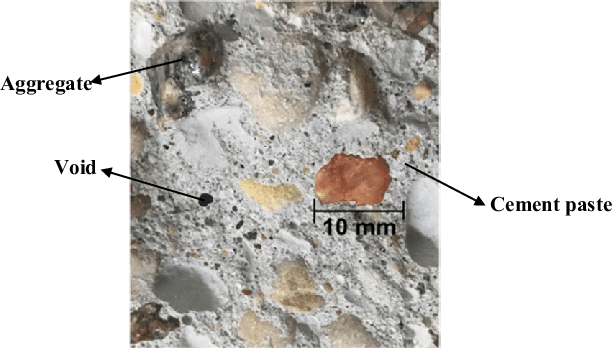
\includegraphics[scale=0.5]{gambar/voidOnConcrete.png}
  \caption{Bentuk Cavities pada Beton Kering \parencite{voidOnConcrete}.}
  \label{fig:voidOnConcrete}
\end{figure}

\section{Ground Penetrating Radar}
\label{sec:groundPenetratingRadar}

\emph{Ground Penetrating Radar} (GPR) merupakan salah satu metode geofisika dalam mengidentifikasi kondisi bawah permukaan. 
Penggunaan GPR pada awalnya digunakan untuk bahan geologi pada alam. 
Seiring berkembangnya teknologi, GPR dapat diterapkan untuk media jenis lainnya, seperti kayu, beton, dan aspal \parencite{jol2008ground}.

\begin{figure}[ht]
  \centering
  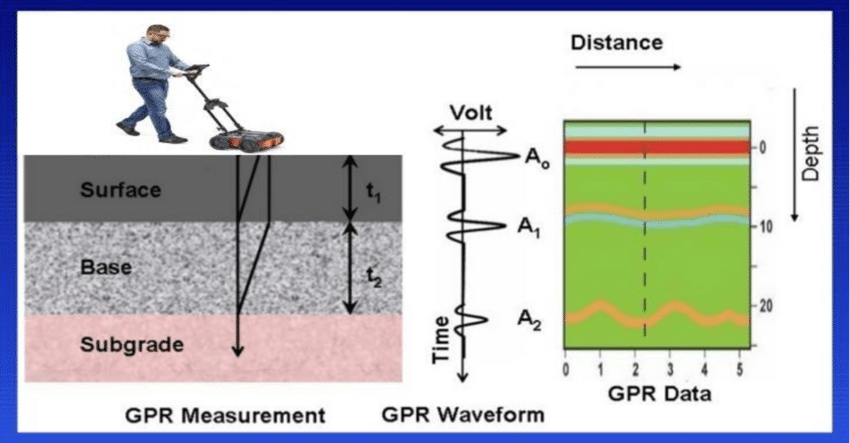
\includegraphics[scale=0.35]{gambar/prinsipGPR.png}
  \caption{Prinsip Kerja GPR Secara Umum \parencite{gprPrinciple}.}
  \label{fig:prinsipGpr}
\end{figure}

GPR terbagi menjadi 2 bagian, yaitu bagian antena pemancar (transmitter) dan bagian antena penerima (receiver). 
Garis besar sistem GPR dapat dilihat pada gambar \ref{fig:prinsipGpr}. 
Antena pemancar dan penerima biasanya identik dan memenuhi karakteristik bentuk gelombang yang dihasilkan. 
Antena pemancar membangkitkan sinyal listrik ke dalam tanah. 
Selama perambatan, sinyal akan mengalami berbagai kerugian (loss). 
Jika sinyal bertabrakan dengan bahan yang tidak homogen dengan media perambatan, maka sinyal akan dipantulkan. 
Sinyal ini akan diterima dan diproses oleh antena penerima.

Perambatan gelombang elektromagnetik diatur oleh sifat dielektrik medium yang dilaluinya, yaitu permitivitas dielektrik ($\varepsilon$), konduktivitas listrik ($\sigma$) dan permeabilitas magnetik ($\mu$). 
Secara khusus, permitivitas dielektrik dan konduktivitas listrik sangat mempengaruhi perilaku gelombang perambatan, masing-masing dalam hal kecepatan gelombang dan atenuasi gelombang, dan permeabilitas magnetik sama untuk semua bahan non-magnetik dengan permeabilitas magnetik ruang bebas $\mu_{0}$ dan tidak mempengaruhi perambatan dari gelombang EM. 
Kedalaman penetrasi dan resolusi spasial dipengaruhi oleh beberapa faktor, di antaranya adalah frekuensi sinyal yang dipancarkan dan jenis material yang diselidiki. \parencite{gprIntroduction}

Secara teoritis, nilai medan elektromagnetik dijelaskan melalui persamaan Maxwell : 

\begin{equation}
  \label{eq:maxWellE}
  \nabla  x \vec{E} = - \frac{ \delta  \vec{B}}{ \delta t} 
\end{equation}

\begin{equation}
  \label{eq:maxWellH}
  \nabla x  \vec{H}  =   \vec{J}  + \frac{ \delta  \vec{D} }{ \delta t} 
\end{equation}

\begin{equation}
  \label{eq:maxWellD}
  \nabla . \vec{D} =  q
\end{equation}

\begin{equation}
  \label{eq:maxWellB}
  \nabla . \vec{B} =  0
\end{equation}

Dimana $\vec{E}$ ($V.m^{-1}$) merupakan vektor kuat medan listrik, q ($C.m^{-3}$) merupakan kerapatan muatan listrik, $\vec{B}$ (T) merupakan vektor kerapatan fluks magnet, $\vec{J}$($A.m^{-2}$) merupakan vektor kerapatan arus listrik, $\vec{D}$ ($C.m^{-2}$) merupakan vektor perpindahan listrik, t (s) merupakan waktu, dan $\vec{H}$ ($A.m^{-1}$) merupakan vektor intensitas medan magnet. \parencite{jol2008ground}

Sebaliknya, perilaku medium tempat gelombang elektromagnetik merambat, dapat dijelaskan oleh hubungan konstitutif. 
Hubungan konstitutif adalah sarana untuk menggambarkan respons material terhadap bidang elektromagnetik. 
Secara matematis, hubungan konstitutif dirumuskan sebagai berikut:
\begin{equation}
  \label{eq:mediumJ}
  \vec{J} =  \sigma \vec{E}
\end{equation}

\begin{equation}
  \label{eq:mediumD}
  \vec{D} =  \varepsilon \vec{E}
\end{equation}

\begin{equation}
  \label{eq:mediumB}
  \vec{B} =  \mu \vec{H}
\end{equation}

Dengan menggabungkan teori medan EM dengan hubungan konstitutif, dimungkinkan untuk menggambarkan sinyal GPR secara komprehensif.


\subsection{GprMax}
\label{subsec:gprMax}

GprMax merupakan open source software yang mensimulasikan propagasi gelombang elektromagnetik. 
GprMax memecahkan persamaan Maxwell dalam 3D menggunakan metode Finite-Difference Time-Domain (FDTD). 
GprMax dirancang untuk pemodelan Ground Penetrating Radar (GPR) tetapi juga dapat digunakan untuk memodelkan propagasi gelombang elektromagnetik untuk banyak aplikasi lainnya. 

\begin{figure}[ht]
  \centering
  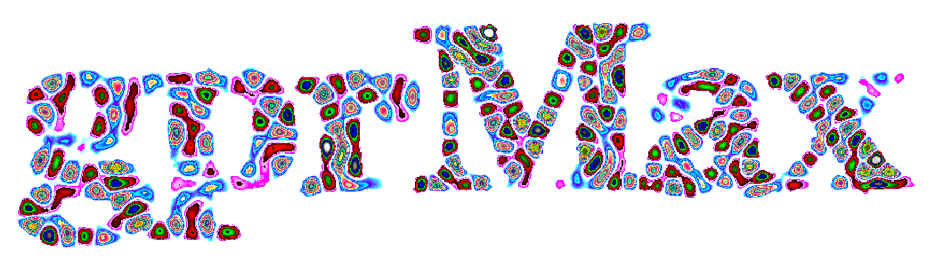
\includegraphics[scale=0.35]{gambar/gprMax.png}
  \caption{Logo gprMax (sumber : www.gprmax.com).}
  \label{fig:logogprMax}
\end{figure}

GprMax saat ini dirilis di bawah GNU General Public License v3 atau lebih tinggi. 
Bahasa pemrograman yang digunakan pada gprMax aslinya berbasis C, dan sekarang sudah sepenuhnya ditulis ulang menggunakan kombinasi bahasa Python dan Cython. 
Hal ini termasuk pemecah berbasis CPU yang diparalelkan menggunakan OpenMP, dan pemecah berbasis GPU yang ditulis menggunakan model pemrograman NVIDIA CUDA. \parencite{gprMax}

\subsection{Pengolahan Sinyal}
\label{subsec:pengolahanSinyal}

Sinyal GPR sangat terkontaminasi oleh \emph{clutter}. 
Pengolahan sinyal pada GPR utamanya merupakan sarana untuk mengurangi \emph{clutter} tersebut. 
Pada dasarnya, rasio dari sinyal terhadap clutter adalah kunci dari deteksi objek. 
Tujuan dari pengolahan sinyal pada GPR adalah untuk menyajikan gambar yang dapat dimengerti, atau mengklasifikasikan hasil target berdasarkan prosedur tertentu. 
Untuk menghasilkan data visual, data GPR akan diproses dan ditampilkan dalam mode A-Scan, B-Scan, atau \emph{C-Scan}. \parencite{3DgprMax}
Ketiga bentuk Mode visualisasi sinyal GPR dapat dilihat pada gambar \ref{fig:scanmodes}

\begin{figure}[ht]
  \centering
  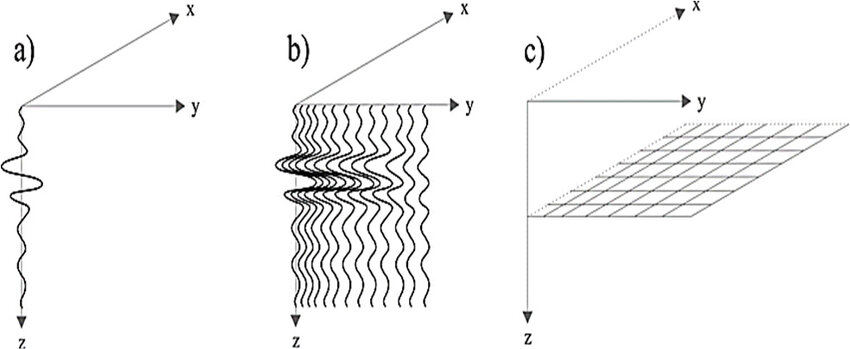
\includegraphics[scale=0.5]{gambar/scanModes.png}
  \caption{Mode visualisasi sinyal GPR: (a) A-scan, (b) B-scan, and (c) C-scan \parencite{scanModes}.}
  \label{fig:scanmodes}
\end{figure}

\subsection{A-Scan}
\label{subsec:aScan}

A-Scan merupakan mode GPR yang ditampilkan dalam satu dimensi, di mana amplitudo gelombang diplot dalam fungsi waktu. 
Pada mode ini, sinyal GPR direkam dan ditampilkan sebagai amplitudo sinyal terhadap waktu. 
Sinyal ini mencerminkan pantulan gelombang elektromagnetik yang terdeteksi oleh GPR saat menjelajahi lapisan tanah atau struktur di bawah permukaan.

Dalam mode A-scan, sumbu waktu merepresentasikan jarak atau posisi relatif dari antena GPR saat menjelajahi lapisan tanah atau struktur di bawah permukaan. 
Titik awal grafik A-scan mengindikasikan saat gelombang elektromagnetik dipancarkan oleh antena GPR, dan titik akhirnya mencerminkan waktu yang dibutuhkan untuk gelombang elektromagnetik mencapai target atau objek bawah permukaan dan kembali ke antena GPR.
Sedangkan Amplitudo sinyal pada sumbu vertikal menunjukkan kekuatan atau intensitas sinyal GPR yang terdeteksi oleh antena saat berinteraksi dengan benda atau lapisan bawah permukaan. 
Puncak amplitudo yang tinggi menunjukkan adanya pantulan kuat, sedangkan amplitudo yang lebih rendah menunjukkan adanya pantulan yang lebih lemah.

Gambar \ref{fig:AscanGPR} merupakan contoh dari grafik A-Scan pada simulasi gprMax yang ditampilkan dalam 6 jenis grafik. 
Untuk setiap barisnya merupakan grafik A-scan berdasarkan sumbu acuan (sumbu-x, sumbu-y, dan sumbu-z), sedangkan setiap kolomnya merupakan grafik A-scan berdasarkan kuat bidang elektromagnetik (kuat medan listrik (E) dan kuat medan magnet (H))
Pada grafik, terlihat grafik sinyal A-scan untuk kuat medan listrik pada sumbu-x dan sumbu-y, serta kuat medan magnet pada sumbu-z selalu bernilai 0.
Hal ini menunjukkan pada simulasi gprMax, sinyal GPR dipancarkan secara vertikal (sumbu-z) ke arah bawah suatu permukaan.

\begin{figure}[ht]
  \centering
  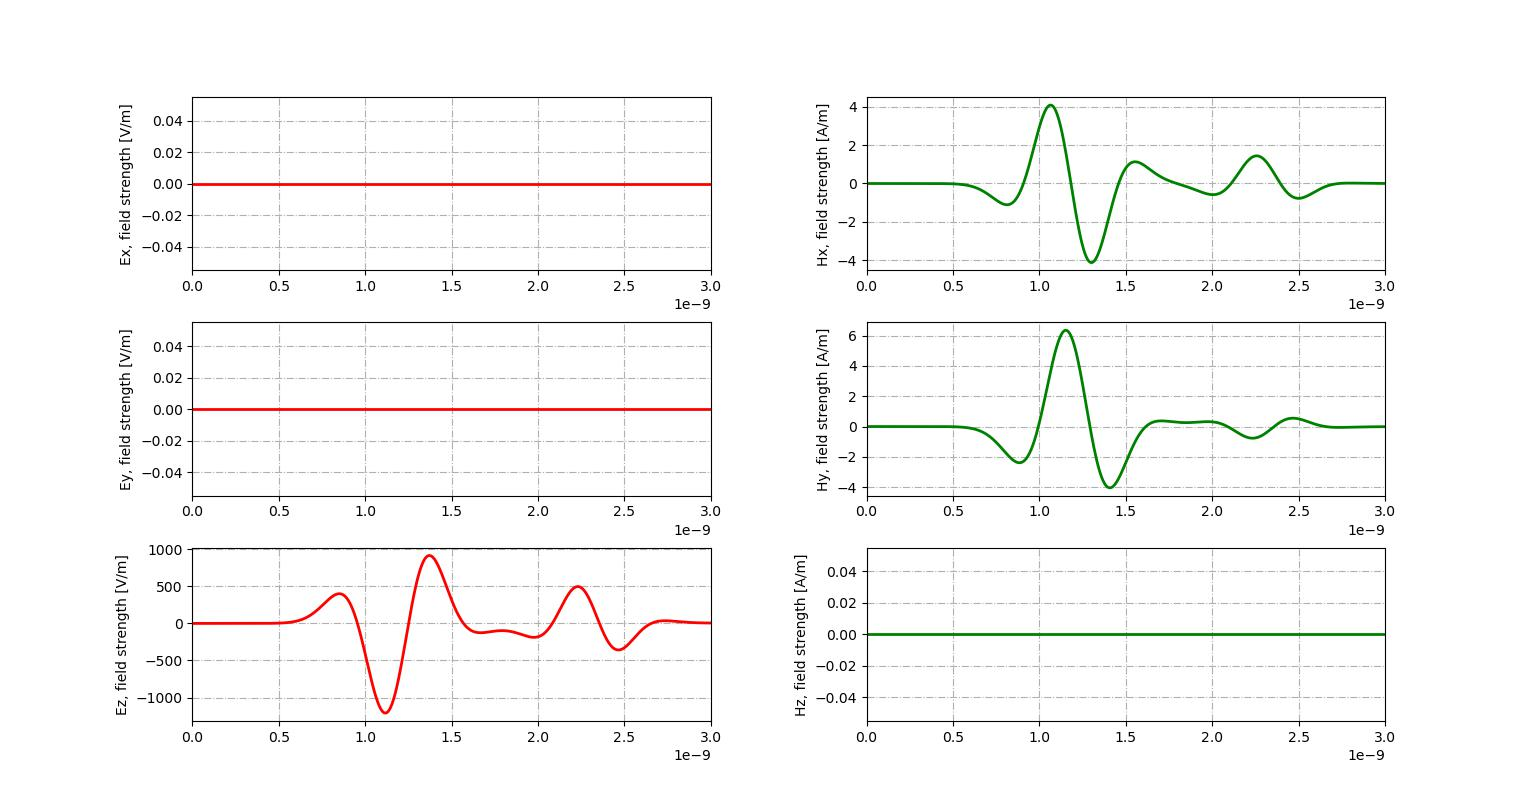
\includegraphics[scale=0.45]{gambar/GPRAscan.jpeg}
  \caption{Contoh A-Scan Sinyal GPR.}
  \label{fig:AscanGPR}
\end{figure}

Bentuk gelombang tunggal atau A-Scan didefinisikan sebagai

\begin{equation}
  \label{eq:Ascan}
  F(z)=A( x_{i} , y_{j} , z_{k} )
\end{equation}

di mana rentang k = 1 sampai N, i dan j bilangan konstan \parencite{danielDvd}.\\

\subsection{B-Scan}
\label{subsec:bScan}

B-scan merupakan sebuah set dari gelombang A-scan GPR yang berurutan sepanjang arah tertentu. 
Mode B-scan menghasilkan gambar 2 dimensi dari data GPR, yang berguna untuk memberikan gambaran keseluruhan dari struktur yang dilintasi oleh GPR.
Dengan melihat gambar B-scan, pengguna GPR dapat mengidentifikasi batas lapisan, perubahan komposisi material, atau adanya objek tertanam seperti pipa, kabel, atau struktur bawah permukaan lainnya.

Dalam mode B-scan, sumbu horizontal pada gambar menunjukkan posisi lintasan perangkat GPR saat pemindaian, sedangkan sumbu vertikal merepresentasikan kedalaman atau jarak relatif. 
Setiap titik pada gambar B-scan mewakili amplitudo atau kekuatan sinyal GPR yang terdeteksi pada posisi tersebut. 
Gambar B-scan biasanya ditampilkan dalam skala abu-abu atau dalam warna dengan gradasi intensitas yang menggambarkan kekuatan sinyal.

\begin{figure}[ht]
  \centering
  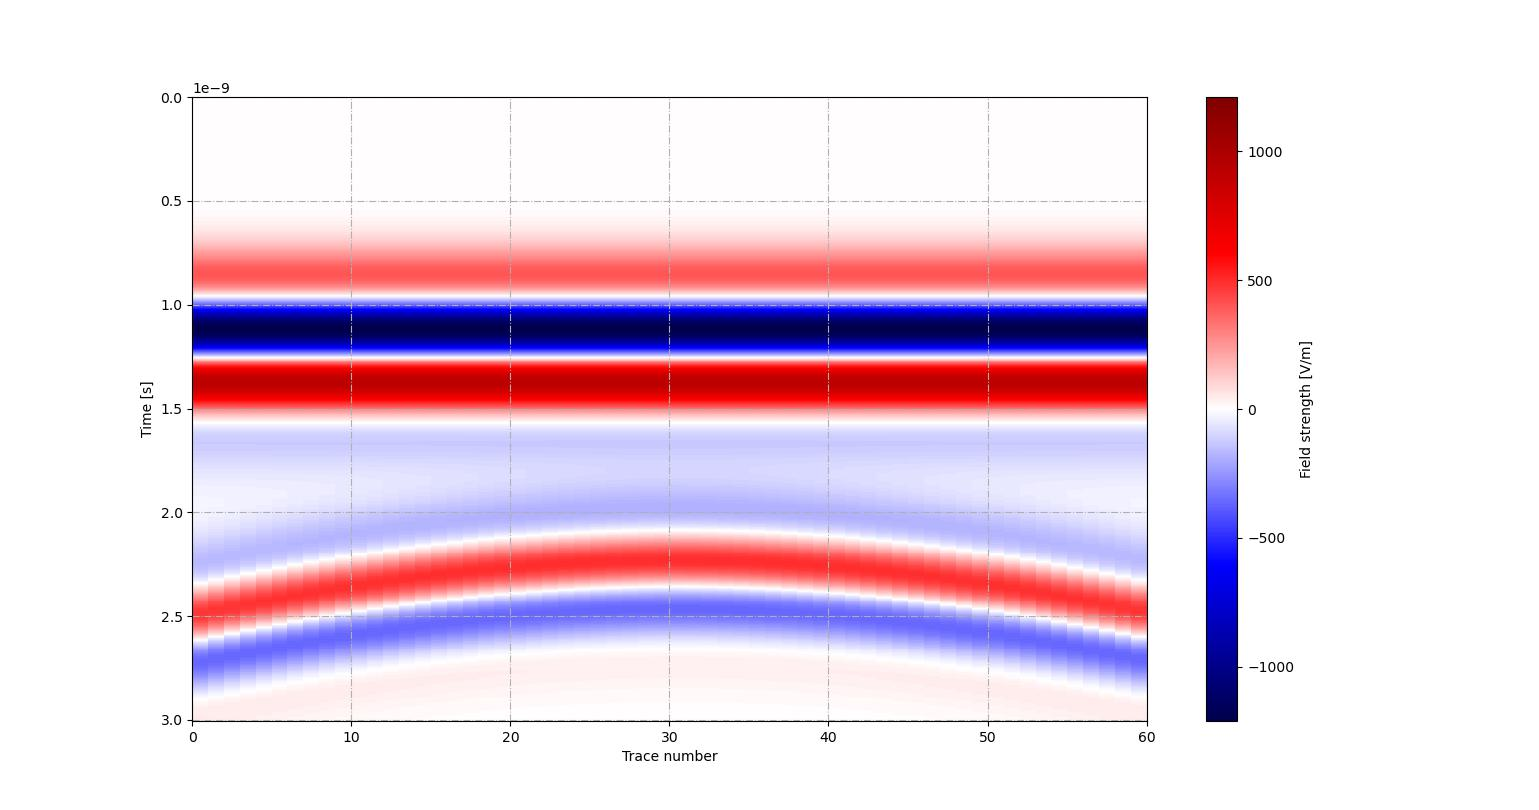
\includegraphics[scale=0.45]{gambar/GPRBscan.jpg}
  \caption{Contoh B-Scan Sinyal GPR.}
  \label{fig:BscanGPR}
\end{figure}

Gambar \ref{fig:BscanGPR} merupakan contoh dari bentuk B-Scan pada simulasi gprMax. 
Gambar B-scan ditampilkan berwarna dengan gradasi warna merah-biru. 
Pada keterangan gradasi warna gambar, warna merah menunjukkan sinyal kuat (nilai positif) dan warna biru menunjukkan sinyal lemah (nilai negatif) dengan interval nilai medan listrik (Ez) dari -1000 $V.m^{-1}$ hingga 1000 $V.m^{-1}$.

Dalam gambar B-scan, bentuk parabola sinyal muncul karena adanya perbedaan konduktivitas atau dielektrik antara lapisan atau objek yang terdeteksi. 
Ketika gelombang elektromagnetik melewati batas antara dua bahan yang berbeda, terjadi pembiasan dan perubahan arah lintasan gelombang.
Hal ini mengakibatkan adanya variasi amplitudo sinyal yang terdeteksi.

Pada gambar \ref{fig:BscanGPR}, perubahan warna merah-biru dan kebalikannya pada sinyal B-scan biasanya mewakili perubahan amplitudo atau kekuatan sinyal yang terdeteksi oleh GPR. 
Perubahan warna ini dapat disebabkan oleh beberapa faktor, yaitu : 

\begin{enumerate}[nolistsep]

  \item Perbedaan konduktivitas material.
  
  Material dengan konduktivitas yang lebih tinggi atau kemampuan untuk memantulkan gelombang elektromagnetik secara lebih baik akan menghasilkan sinyal yang lebih kuat dan warna yang lebih terang (merah) dalam gambar B-scan. 
  Sebaliknya, material dengan konduktivitas rendah atau kemampuan refleksi yang lebih rendah akan menghasilkan sinyal yang lebih lemah dan warna yang lebih gelap (biru).   

  \item Perbedaan bentuk geometri objek.
  
  Objek dengan bentuk yang mengarahkan atau memfokuskan gelombang elektromagnetik ke antena GPR dapat menghasilkan sinyal yang lebih kuat dan warna yang lebih terang (merah). 
  Sebaliknya, objek dengan geometri yang mengakibatkan penyebaran atau dispersi gelombang elektromagnetik akan menghasilkan sinyal yang lebih lemah dan warna yang lebih gelap (biru).

  \item Jarak tempuh gelombang.
  
  Semakin jauh jarak tempuh gelombang elektromagnetik, semakin lemah intensitas sinyal yang terdeteksi. 
\end{enumerate}

Bentuk gelombang dua dimensi atau B-Scan didefinisikan sebagai

\begin{equation}
  \label{eq:Bscanx}
  F(x,z)=A( x_{i} , y_{j} , z_{k} )
\end{equation}

di mana rentang k = 1 sampai N, i = 1 sampai L, dan j bilangan konstan, atau

\begin{equation}
  \label{eq:Bscany}
  F(y,z)=A( x_{i} , y_{j} , z_{k} )
\end{equation}

di mana rentang k = 1 sampai N, j = 1 sampai M, dan i bilangan konstan \parencite{danielDvd}.

\subsection{Migrasi}
\label{subsec:migrasi}

Migrasi merupakan teknik pemrosesan data GPR untuk meningkatkan resolusi spasial dan mengembangkan gambar bawah permukaan yang lebih realistis \parencite{jol2008ground}.
Migrasi akan mengubah data mentah GPR yang tidak terfokus menjadi gambar terfokus yang menunjukkan lokasi dan ukuran objek yang sebenarnya dengan reflektifitas elektromagnetik yang sesuai.
Metode migrasi paling populer dan fungsional untuk aplikasi pencitraan GPR antara lain \emph{hyperbolic summation}, \emph{Kirchhoff's migration}, \emph{phase-shift migration}, \emph{$\omega-k$ (Stolt) migration}, dan \emph{back-projection focusing} \parencite{Ozdemir2014ARO}.
Contoh hasil migrasi sinyal B-scan GPR sederhana dapat dilihat pada gambar \ref{fig:migrasiGPR}.

\begin{figure}[ht]
  \centering
  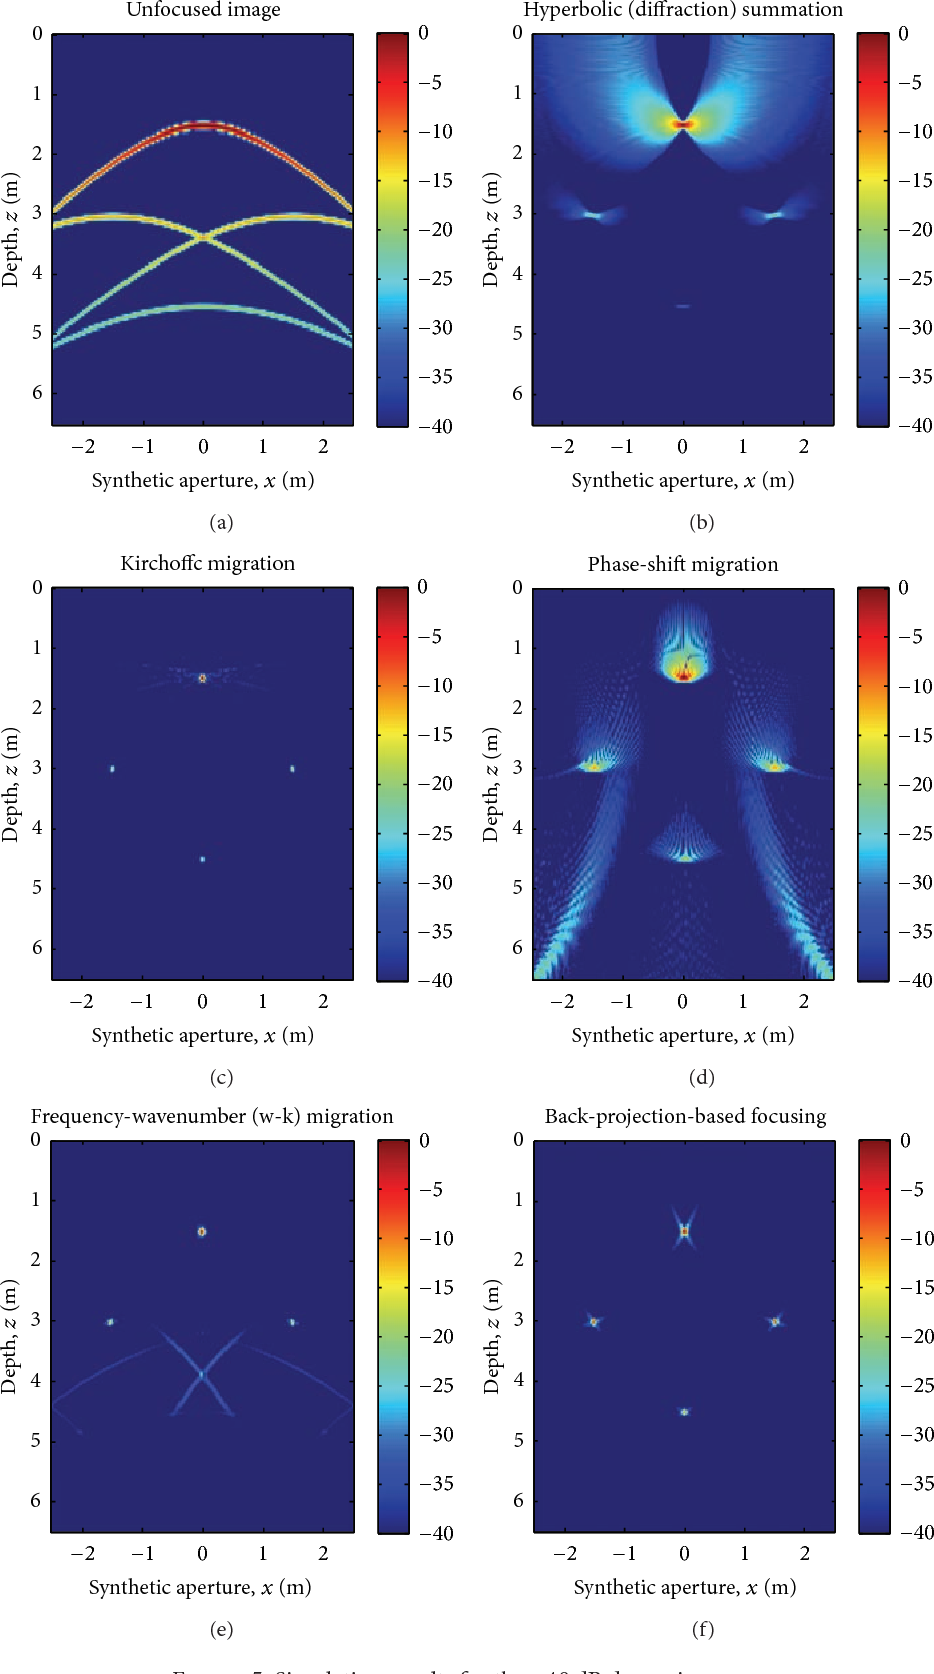
\includegraphics[scale=0.27]{gambar/migrasi.png}
  \caption{Contoh Migrasi Sinyal B-Scan GPR \parencite{Ozdemir2014ARO}.}
  \label{fig:migrasiGPR}
\end{figure}

\subsection{Bandwidth}
\label{subsec:bandwidth}

\emph{Bandwidth} merupakan perbedaan antara batas frekuensi tertinggi dengan frekuensi terendah sinyal. 
Pengukuran \emph{Bandwidth} berhubungan langsung dengan resolusi. 
Durasi waktu dari pulsa transmisi berbanding terbalik dengan \emph{bandwidth}. 
Secara matematis, nilai \emph{bandwidth} dan durasi waktu dapat didefinisikan sebagai berikut

\begin{equation}
  \label{eq:BW}
  B \geq  \frac{v}{4 \Delta r} 
\end{equation}

di mana r merupakan panjang resolusi dan v merupakan kecepatan perambatan \parencite{jol2008ground}.

\subsection{Center Frequency}
\label{subsec:centerFrequency}

\emph{Center frequency} merupakan titik tengah dari batas frekuensi atas dan frekuensi bawah. 
\emph{Bandwidth} tidak menentukan frekuensi dari sinyal GPR, namun \emph{bandwidth} dapat menentukan batas frekuensi dari \emph{center frequency}.
Semakin rendah frekuensi, semakin besar kemungkinan mendapat sinyal GPR dari media perambatnya.

Sinyal GPR dicirikan oleh rasio bandwidth terhadap \emph{center frequency}

\begin{equation}
  \label{eq:cF}
  R =  \frac{B}{ f_{c} } 
\end{equation}

di mana rasio R diusakan sebesar mungkin \parencite{jol2008ground}. 
Umumnya GPR mencapai rasio R mendekati 1, sehingga \emph{bandwidth} biasa ditafsirkan bernilai sama dengan nilai \emph{center frequency}.

\subsection{Ricker Wavelet}
\label{subsec:rickerWavelet}

Pada GPR, metode pembangkitan data Ricker Wavelet merupakan salah satu metode terbaik dalam membangkitkan data seismik \parencite{rickeronSeismic}. 
Wavelet merupakan satu gelombang pendek, yang diperoleh dari suatu model matematik. 
Wavelet Ricker memungkinkan untuk menggunakan sedikit parameter dalam mendeteksi sinyal seismik.

Ricker wavelet didefinisikan dalam domain waktu sebagai

\begin{equation}
  \label{eq:rickerTimeDomain}
  r(t) =  \big(1 -  \frac{1}{2} (  \omega _{p} ^{2}  t^{2} ) \big)  . exp \big(- \frac{1}{4} ( \omega _{p} ^{2}  t^{2} ) \big) 
\end{equation}

di mana t merupakan waktu dan $\omega_{p}$ merupakan frekuensi sudut puncak.

Spektrum frekuensi dari ricker wavelet dapat didefinisikan sebagai

\begin{equation}
  \label{eq:rickerTimeDomain}
  R( \omega ) =  \big( \frac{2 \omega ^{2}}{  \sqrt{ \pi }  \omega _{p} ^{3}} \big)  . exp \big(- \frac{ \omega ^{2}}{ \omega _{p} ^{2}} \big) 
\end{equation}

\begin{figure}[ht]
  \centering
  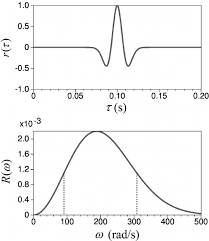
\includegraphics[scale=1]{gambar/ricker.jpg}
  \caption{Grafik gelombang ricker beserta spektrum frekuensi \parencite{rickerWavelet}.}
  \label{fig:gelombangRicker}
\end{figure}

Grafik ricker wavelet beserta spektrum frekuensi ditampilkan pada gambar \ref{fig:gelombangRicker}. 
Pada gambar tersebut, digunakan frekuensi sudut puncak $\omega$ = 60$\pi$ rad/s

\section{Neural Networks}
\label{sec:neuralNetworks}

\emph{Neural Network} merupakan salah satu bagian dari \emph{machine learning} yang terinspirasi dari bentuk jaringan neuron pada otak manusia. 
Setiap neuron atau node akan dikumpulkan dalam suatu lapisan (\emph{layers}), yang akan saling berhubungan dan berurutan. 
Pada tingkat paling dasarnya, sebuah jaringan terdiri dari satu node yang mengambil input vektor dikali bobot tertentu, kemudian diubah dengan transformasi non-linear untuk mencapai output yang diharapkan. 
Jaringan juga memiliki lapisan tersembunyi (\emph{hidden layers}), yang beratnya dapat dioptimalkan dalam mencapai output yang diharapkan.

\subsection{Deep Learning}
\label{subsesc:deeplearning}
\emph{Deep learning} merupakan algoritma yang menggunakan \emph{artificial neural networks} (ANN). 
ANN kemungkinan dianggap sebagai cara yang paling baik dalam menentukan serangkaian fungsi yang fleksibel. 
Hal ini dikarenakan ANN dibangun dari banyak blok komputasi dasar yang disebut neuron. 
Secara khusus, daripada memprogram serangkaian instruksi khusus untuk menyelesaikan masalah secara langsung, model \emph{deep learning} dilatih berdasarkan data dari dunia nyata dan mempelajari bagaimana cara menyelesaikan masalah \parencite{PDLT-2022}. 

\subsection{Convolutional Neural Network}
\label{subsec:convolutionalNeuralNetwork}

Dalam \emph{deep learning}, \emph{Convolutional Neural Network} (CNN) adalah kelas jaringan saraf tiruan yang paling umum diterapkan untuk menganalisis citra visual. 
Convolutional Neural Network (CNN) telah menunjukkan kinerja yang sangat baik dalam banyak masalah visi komputer dan \emph{machine learning}. 
Banyak paper yang telah diterbitkan tentang topik ini, dan beberapa \emph{open source software} CNN telah tersedia. 
CNN berguna dalam banyak aplikasi, terutama dalam tugas-tugas terkait gambar. 
Aplikasi CNN termasuk klasifikasi gambar, segmentasi semantik gambar, deteksi objek dalam gambar, dsb \parencite{introductionCNN}. 

\section{Model Generatif}
\label{sec:modelGeneratif}

Model generatif merupakan bagian dari \emph{Neural Network} yang memungkinkan upaya sintesis dara yang realistis. 
Dasar dari model ini terletak pada \emph{neural network} yang berfungsi secara universal. 
Model ini memungkinkan model, yang awalnya diberi input, mempelajari fitur dari input tersebut, kemudian mampu menghasilkan output yang mirip dengan data input.

\subsection{Generative Adversarial Network}
\label{subsec:generativeAdversarialNetwork}

\emph{Generative Adversarial Network} (GAN) adalah bentuk model generatif, di mana model dibagi menjadi 2 bagian, yaitu bagian generatif (G) dan bagian diskriminator (D). 
Bagian generatif merupakan bagian untuk mensintesis data, sedangkan bagian diskriminator merupakan bagian untuk menentukan apakah data sintesis merupakan data palsu atau asli. 
Model ini seringkali diaplikasikan untuk mereplikasi suatu data, seperti gambar, video, dan audio.

Generator dan Diskriminator akan saling menguntung-rugikan, dengan fungsi V(D,G) direpresentasikan sebagai berikut : 

\begin{equation}
  \label{eq:GAN}
  min_{G} max_{D} V(G,D) =  E_{x \sim p_{data} (x)} \big[ log D(x) \big] + E_{z \sim p_{z} (z)} \big[ log  \big(1-D \big(G(z)\big) \big) \big]
\end{equation}

Dalam mempelajari distribusi generator p pada data x, variabel kebisingan input pz(z) didefinisikan sebelumnya, kemudian pemetaan direpresentasikan ke ruang data sebagai G(z; (teta)g), di mana G adalah fungsi diferensiasi yang direpresentasikan oleh multilayer perceptron dengan parameter (teta)g. 
Multilayer perceptron (MLP) kedua D(x; (teta)d) yang menghasilkan skalar tunggal juga didefinisikan. 
D(x) merepresentasikan kemungkinan bahwa x berasal dari data daripada pg. 
Diskriminator dilatih untuk memaksimalkan kemungkinan menempatkan label yang benar untuk data pelatihan dan sampel dari Generator. 
Generator dan  Diskriminator dilatih secara bersamaan untuk meminimalkan log(1-D(G(z))). \parencite{GAN}

\subsection{Conditional Generative Adversarial Network}
\label{subsec:conditionalGAN}

\emph{Generative Adversarial Network} dapat diperluas ke model bersyarat jika generator dan diskriminator dikondisikan pada beberapa informasi tambahan y. 
Konstanta y bisa berupa segala jenis informasi tambahan, seperti label kelas atau data dari modalitas lain. 
Pengkondisian juga dapat dilakukan dengan memasukkan y ke dalam diskriminator dan generator sebagai lapisan masukan tambahan.

Fungsi dari untung rugi Generator dan Diskriminator V(D,G) untuk \emph{Conditional Generative Adversarial Network} (CGAN) direpresentasikan sebagai berikut :

\begin{equation}
  \label{eq:CGAN}
  min_{G} max_{D} V(G,D) =  E_{x \sim p_{data} (x)} \big[ log D(x|y) \big] + E_{z \sim p_{z} (z)} \big[ log  \big(1-D \big(G(z|y)\big) \big) \big]
\end{equation}

Dalam generator, input kebisingan sebelumnya, pz(z), dan y digabungkan dalam representasi tersembunyi gabungan, dan kerangka pelatihan adversarial memungkinkan fleksibilitas yang cukup besar dalam bagaimana representasi tersembunyi ini disusun. 
Dalam diskriminator x dan y disajikan sebagai input dan ke fungsi diskriminatif (dalam kasus ini diwujudkan kembali oleh MLP). \parencite{CGAN}

\section{Loss Function}
\label{sec:lossFunction}

\emph{Loss Function} merupakan fungsi yang membandingkan target dengan nilai output yang diprediksi. 
Fungsi ini mengukur seberapa baik suatu \emph{Neural Network} memodelkan data pelatihan. 
Saat pelatihan, model akan meminimalkan nilai \emph{Loss Function} antara output yang diprediksi dan target.

\subsection{Sigmoid Cross-Entropy Loss}
\label{sigmoidCrossEntropyLoss}

\emph{Sigmoid function} merupakan fungsi kontinu berbentuk “S” dengan range dari 0 sampai 1 untuk domain bilangan riil. 
Fungsi sigmoid adalah fungsi yang paling umum dikenal digunakan dalam \emph{Feedforward Neural Network} (FNN) karena sifat nonlinier dan kesederhanaan komputasi turunannya. 
Bentuk sederhana dari fungsi sigmoid secara matematis didefinisikan sebagai 

\begin{equation}
  \label{eq:sigmoid}
  f(h) =  \frac{1}{1+exp(-2 \beta h)} 
\end{equation}

dimana $\beta$ merupakan konstanta atau parameter yang dapat dilatih dan fungsi memenuhi kondisi f(h) + f(-h) = 1 \parencite{sigmoid}. Bentuk grafik fungsi sigmoid dapat dilihat pada gambar \ref{fig:sigmoid}

\begin{figure}[ht]
  \centering
  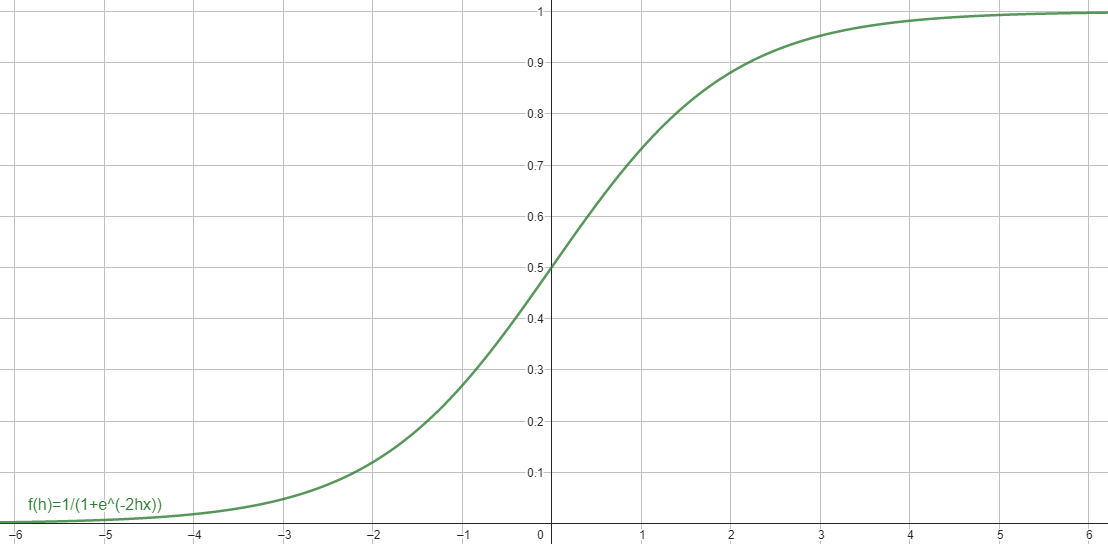
\includegraphics[scale=0.35]{gambar/sigmoid.png}
  \caption{Grafik Fungsi Sigmoid.}
  \label{fig:sigmoid}
\end{figure}

\emph{Sigmoid cross-entropy loss}, juga dikenal sebagai \emph{binary cross-entropy loss} \parencite{lossFunction}, merupakan fungsi yang digunakan untuk mengukur perbedaan antara prediksi yang dihasilkan oleh model dan label yang sebenarnya pada kasus klasifikasi biner, di mana setiap sampel data hanya dapat memiliki dua kelas yang mungkin. 
Fungsi \emph{sigmoid cross-entropy loss} menggunakan fungsi sigmoid untuk memetakan nilai prediksi yang kontinu ke dalam rentang antara 0 dan 1. 
Selanjutnya, fungsi ini membandingkan nilai prediksi yang dihasilkan dengan label yang sebenarnya menggunakan matriks \emph{loss cross-entropy}. 
Secara matematis, fungsi \emph{sigmoid cross-entropy loss} didefinisikan sebagai 

\begin{equation}
  \label{eq:sigmoidCrossEntropyLoss}
  L_{log} = H(f,y) = - \frac{1}{N}  \sum_ {i=1} ^N  \big( y_{i} . log \big(f( y_{i} ) \big) +(1 - y_{i}) . log \big(1 - f( y_{i} ) \big) \big)  
\end{equation}

dimana $y_{i}$ merupakan label untuk titik tertentu (0 untuk warna hijau dan 1 untuk warna merah) dan f(y) merupakan fungsi sigmoid untuk memprediksi probabilitas suatu titik bernilai 0 (hijau) untuk semua titik N.

\subsection{Image Differencing}
\label{imagediff}

\emph{Image differencing} merupakan metode pengurangan nilai digital dari suatu gambar dengan gambar lain. 
Metode ini akan mengurangi nilai setiap piksel gambar yang berada di posisi yang sama, kemudian hasil pengurangan akan ditampilkan dalam bentuk gambar. 
Secara matematis, metode image differencing didefinisikan sebagai

\begin{equation}
  \label{eq:imagediff}
  l_{d}(x,y) =  l_{1}(x,y) - l_{2}(x,y) 
\end{equation}

dimana $l_{1}$ dan $l_{2}$ merupakan kedua gambar input dan (x,y) merupakan posisi pixel \parencite{imgdiff}.

\subsection{Mean Squared Error}
\label{subsec:MSE}

\emph{Mean Squared Error} (MSE) adalah rata-rata error kuadrat antara nilai aktual dan prediksi. 
Dalam model yang memprediksi variabel kontinu, MSE adalah tolok ukur kinerja yang ideal karena keterkaitannya dengan konsep \emph{cross-entropy} dari teori informasi. 
\emph{Cross-entropy} akan mengukur kesamaan dua distribusi probabilitas. 
Jika tujuan pemodelan adalah untuk mengidentifikasi model yang paling dekat mereproduksi distribusi penghasil data yang sebenarnya, maka model terbaik akan meminimalkan \emph{cross-entropy} antara prediksi model dan data pelatihan \parencite{MSE}. 

\subsection{Structural Similarity Index Measurement}
\label{subsec:SSIM}

\emph{Structural Similarity Index Measurement} (SSIM) adalah metode yang digunakan untuk mengukur kesamaan struktural antara dua gambar atau sinyal. 
Metrik ini dikembangkan untuk mencerminkan persepsi visual manusia dalam mengevaluasi kesamaan antara dua gambar. 
SSIM memperhitungkan 3 parameter yang ada pada citra, yaitu kecerahan (\emph{luminance}), kontras (\emph{contrast}), dan struktur (\emph{structure}). 
Diagram sistem SSIM dapat dilihat pada gambar \ref{fig:SSIM}.

\begin{figure}[ht]
  \centering
  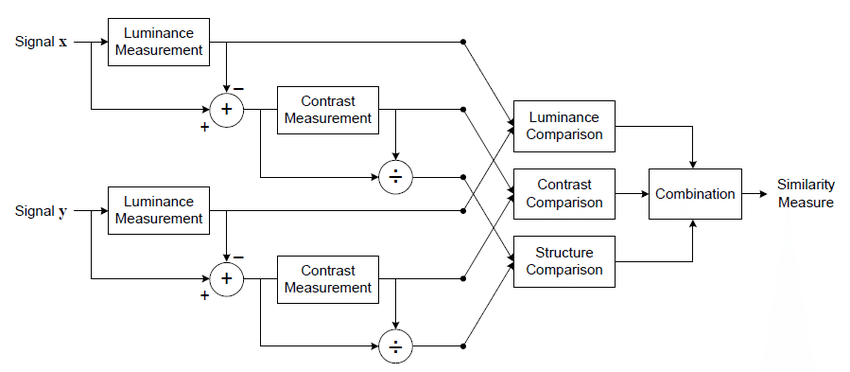
\includegraphics[scale=0.5]{gambar/SSIM.png}
  \caption{Diagram Sistem SSIM \parencite{SSIM}.}
  \label{fig:SSIM}
\end{figure}

Secara matematis, nilai SSIM dari 2 gambar (x, y) didefinisikan sebagai 

\begin{equation}
  \label{eq:ssim1}
  SSIM(x,y) =  [l(x,y)^{ \alpha } ] . [c(x,y)^{ \beta }].[s(x,y)^{ \gamma }]
\end{equation}

dimana $\alpha$, $\beta$ dan $\gamma$ bilangan positif yang merupakan parameter yang digunakan untuk menyesuaikan tingkat kepentingan relatif dari ketiga komponen tersebut. 
Dengan mengasumsikan ketiga komponen memiliki tingkat kepentingan yang sama ($\alpha$=$\beta$=$\gamma$=1), maka nilai SSIM secara spesifik didefinisikan sebagai 

\begin{equation}
  \label{eq:ssim2}
  SSIM(x,y) =  \frac{(2  \mu_{x} \mu_{y} + C_{1})(2 \sigma_{xy} + C_{2} )}{(\mu_{x}^{2}  + \mu_{y}^{2}+C_{1})(\sigma_{x}^{2}+\sigma_{y}^{2}+C_{2})} 
\end{equation}

dimana $\mu$ merupakan nilai rata-rata dari intensitas piksel, $\sigma$ merupakan estimasi dari kontras gambar, dan C1 C2 merupakan konstanta untuk menghindari ketidakstabilan \parencite{SSIM}.

\section{Adam Optimizer}
\label{adamOptimizer}

Adam merupakan sebuah metode untuk optimasi stokastik yang efisien, yang hanya membutuhkan gradien orde pertama dengan sedikit kebutuhan memori. 
Nama Adam diambil dari singkatan \emph{adaptive moment estimation}. 
Metode ini mudah diimplementasikan, efisien secara komputasi, memiliki sedikit kebutuhan memori, tidak berubah terhadap penskalaan diagonal gradien, dan cocok untuk masalah yang besar dalam hal data dan/atau parameter. 
Metode ini merupakan gabungan dari dua metode, yaitu AdaGrad \parencite{adaGrad}, yang bekerja dengan baik dengan gradien sparse, 
dan RMSProp \parencite{RMSProp}, yang bekerja dengan baik di pengaturan \emph{on-line} dan \emph{non-stationary}\parencite{adam}.
\cleardoublepage

% Bab 3 desain dan implementasi
\chapter{METODOLOGI}
\label{chap:metodologi}

\section{Metode yang digunakan}
\label{sec:metode}

Penelitian ini dilaksanakan sesuai dengan metodologi yang telah dirancang. 
Metodologi terbagi menjadi 4 tahap, yaitu pengumpulan data, pembentukan arsitektur GAN, training model, dan evaluasi model. 
Gambar \ref{fig:metodologi} menunjukkan diagram dari metodologi penelitian.

\begin{figure}[ht]
  \centering
  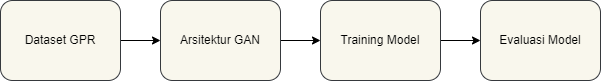
\includegraphics[scale=0.7]{gambar/metodologi.png}
  \caption{Diagram Metodologi Penelitian}
  \label{fig:metodologi}
\end{figure}

\subsection{Dataset GPR}
\label{subsec:datasetgpr}

Tahap ini merupakan tahap pengumpulan dataset GPR. 
Data yang dibutuhkan ada 2 jenis, yaitu data input berupa gambar B-scan GPR hasil simulasi gprMax dan data output yang diharapkan berupa gambar bentuk geometri dari gambar B-scan GPR. 
Alur dari proses pengumpulan dataset ditampilkan pada gambar \ref{fig:datasetgpr}.

\begin{figure}[ht]
  \centering
  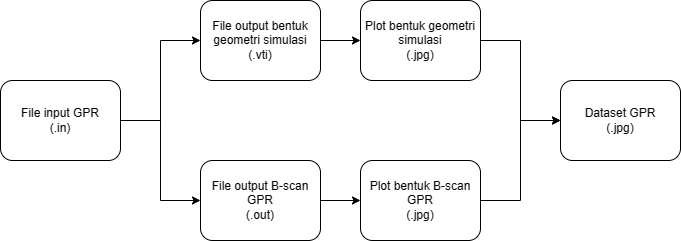
\includegraphics[scale=0.7]{gambar/alur pengumpulan data.png}
  \caption{Diagram Pengumpulan Dataset GPR}
  \label{fig:datasetgpr}
\end{figure}

Simulasi menggunakan gprMax untuk menghasilkan file output bentuk geometri simulasi dan file output B-scan GPR dengan menggunakan file input gprMax. 
Setiap kebutuhan dan cara instalasi gprMax dapat diperoleh di github gprMax. 
Dalam memasang gprMax, dibutuhkan untuk memasang Python, Miniconda/Anaconda, dan C Compiler yang mendukung OpenMP (Desktop development with C++ pada Visual Studio untuk OS Windows). \\

Dalam menyusun kode program input GPR, dibutuhkan beberapa parameter penyusun yang perlu diperhatikan. 
Parameter penyusun tersebut dapat dilihat pada panduan gprMax di website resmi gprMax. 
Pada penelitian ini, parameter sistem yang dibuat pada dataset GPR dapat dilihat pada tabel \ref{tb:inputGPR}. 
Contoh penggunaan parameter pada file input juga dapat dilihat pada gambar \ref{fig:inputgprMax}.

\begin{longtable}{|c|c|c|}
  \caption{Parameter Input GprMax}
  \label{tb:inputGPR}                                   \\
  \hline
  \rowcolor[HTML]{C0C0C0}
  \textbf{Parameter} & \textbf{Nilai} \\
  \hline
  Dimensi                     & 0.3 m x 0.3 m x 0.001 m                   \\
  Jendela Waktu               & 3 ns                                      \\
  Material                    & Beton (medium) dan ruang kosong (objek)   \\
  Basis Sinyal                & Ricker                                    \\
  Arah Laju Sumber Sinyal     & 0.001 m/step terhadap sumbu-X             \\
  Bentuk Objek                & Tabung                                    \\
  \hline
\end{longtable}

\begin{figure}[ht]
  \centering
  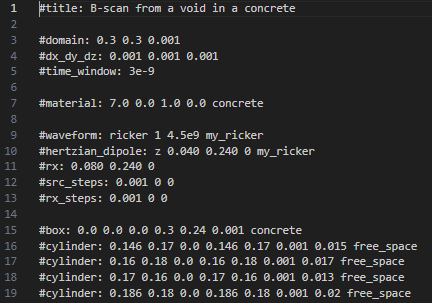
\includegraphics[scale=1]{gambar/inputGprMax.png}
  \caption{Contoh isi file input gprMax}
  \label{fig:inputgprMax}
\end{figure}

Data input gprMax di atas kemudian disimulasikan dengan 2 tools berbeda untuk menghasilkan file output bentuk geometri simulasi dan file output B-scan GPR. 
Dari proses simulasi, diperoleh dua buah hasil, yaitu file output bentuk geometri simulasi (.vti) dan file output B-scan GPR (.out). 
Untuk memperoleh gambar bentuk geometri simulasi, file output bentuk geometri simulasi dijalankan menggunakan aplikasi Paraview. 
Sedangkan untuk memperoleh gambar bentuk sinyal B-scan GPR, file output B-scan GPR dijalankan menggunakan tools dari gprMax.

Kedua jenis gambar ini kemudian digabung menjadi satu gambar dengan menggunakan library PIL. 
Kedua gambar akan disusun horizontal, dimana gambar yang kiri berupa gambar B-scan gprMax dan gambar yang kanan berupa gambar bentuk geometrinya. 
Contoh gabungan gambar ditampilkan pada gambar \ref{fig:contohdata}. 
Gambar hasil gabungan ini yang kemudian menjadi dataset model GAN yang akan dibentuk, yang dalam penelitian ini menggunakan sejumlah 200 data.

\begin{figure}[ht]
  \centering
  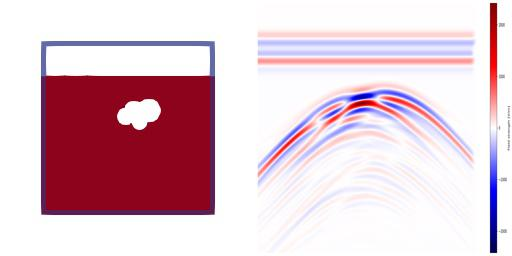
\includegraphics[scale=0.7]{gambar/data1.jpg}
  \caption{Gambar gabungan bentuk geometri bawah permukaan (kiri) dengan bentuk B-scan GPR hasil simulasi (kanan)}
  \label{fig:contohdata}
\end{figure}

\subsection{Arsitektur GAN}
\label{subsec:arsitekturGAN}

Setelah dataset berhasil dikumpulkan, selanjutnya akan dibentuk model dari GAN. 
Model GAN yang akan dibentuk menggunakan model Conditional GAN Pix2pix. 
Arsitektur GAN akan dibagi menjadi 2 bagian, yaitu bagian generator yang berfungsi untuk mensintesis gambar seperti data asli, dan bagian diskriminator yang berfungsi untuk membedakan antara data asli dengan data hasil sintesis. 
Bentuk arsitektur GAN ditampilkan pada gambar \ref{fig:arsitekturGAN}.

\begin{figure}[ht]
  \centering
  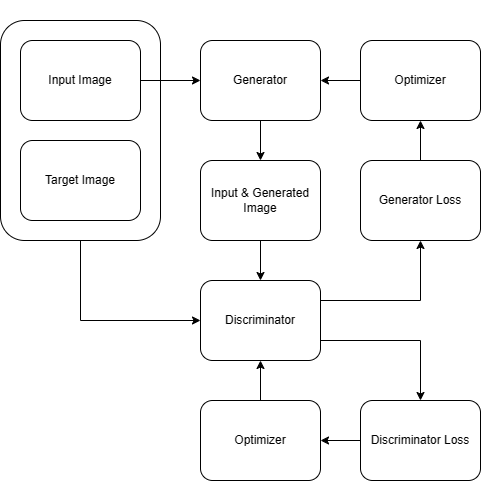
\includegraphics[scale=0.5555]{gambar/Arsitektur GAN.png}
  \caption{Diagram Arsitektur GAN yang Dibentuk}
  \label{fig:arsitekturGAN}
\end{figure}

\newpage

Pada bagian generator, digunakan arsitektur U-net \parencite{UNet}. 
Arsitektur ini terdiri dari jaringan encoder yang dilanjut dengan jaringan decoder. 
Jaringan encoder akan menerapkan proses Convolution $>>$ Batch normalization $>>$ Leaky ReLU. 
Sedangkan decoder akan menerapkan proses Transposed convolution $>>$ Batch normalization $>>$ Dropout (untuk 3 blok pertama) $>>$ ReLU. 
Tiap pasang encoder-decoder memiliki skip connection yang berfungsi untuk menangkap setiap informasi tingkat rendah yang dibagikan antara input dan output. 
Diagram arsitektur Generator dapat dilihat pada gambar \ref{fig:generator}.

\begin{figure}[ht]
  \centering
  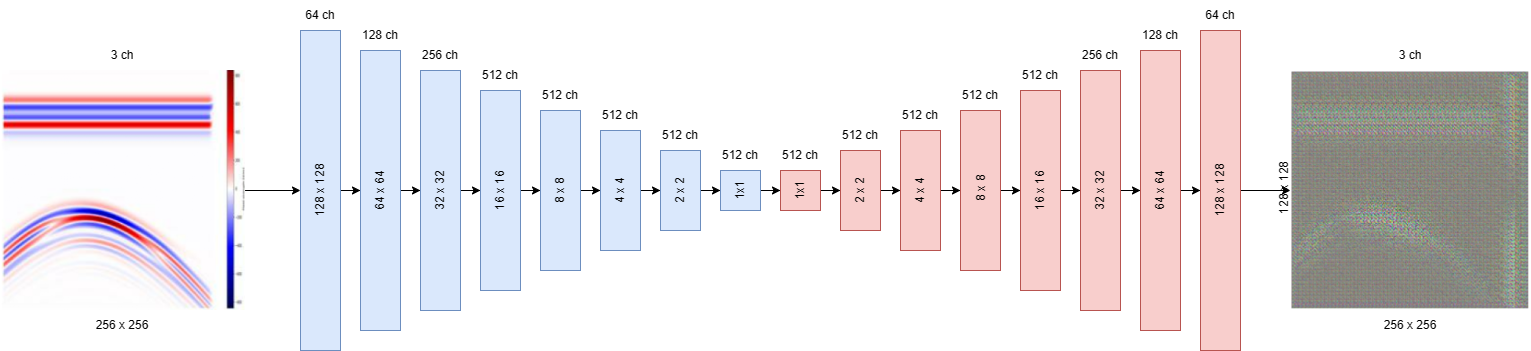
\includegraphics[scale=0.25]{gambar/Generator.png}
  \caption{Diagram Arsitektur Generator}
  \label{fig:generator}
\end{figure}

Pada bagian discriminator, digunakan arsitektur Convolutional Patch GAN yang akan mencoba mengklasifikasikan sepetak (30 x 30) gambar itu nyata atau tidak. 
Discriminator akan menerima dua pasang gambar sebagai input, yaitu gambar input-asli dan gambar input-sintesis. 
Masing-masing pasangan input ini akan digabung terlebih dahulu sebelum masuk ke jaringan encoder. 
Diagram arsitektur Discriminator dapat dilihat pada gambar \ref{fig:discriminator}.

\begin{figure}[ht]
  \centering
  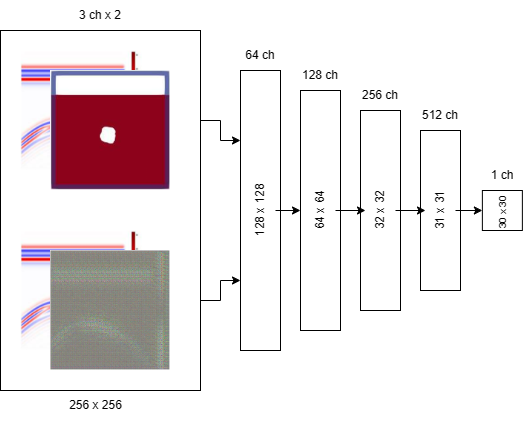
\includegraphics[scale=0.5]{gambar/Discriminator.png}
  \caption{Diagram Arsitektur Discriminator}
  \label{fig:discriminator}
\end{figure}

Generator Loss merupakan gabungan dari sigmoid cross-entropy loss antara gambar yang dihasilkan dengan suatu array 1 (GAN Adversial Loss), dan MAE (Mean Absolute Error) antara gambar yang disintesis dengan gambar asli(L1 Loss). 
Secara matematis, nilai dari Total Generator Loss dapat didefinisikan sebagai 

\begin{equation}
  \label{eq:genLoss}
  Total Generator Loss = GAN Adversial Loss + (Lambda * L1 Loss) 
\end{equation}

dimana Lambda dapat didefisinikan sesuai keinginan model (pada penelitian ini Lambda = 100).

Discriminator Loss terdiri dari sigmoid cross-entropy loss antara gambar asli dengan array 1 (Real Loss), dan sigmoid cross-entropy loss antara gambar yang dihasilkan dengan array 0 (Generated Loss). 
Total Discriminator Loss merupakan jumlah dari Real Loss dan Generated Loss

Pada model GAN juga didefinisikan fungsi optimizer dan checkpoint.
Fungsi optimizer menggunakan Adaptive Moment Estimation (Adam) baik untuk generator maupun diskriminator. 
Fungsi checkpoint digunakan untuk menyimpan hasil sementara (checkpoint) dari hasil pelatihan generator dan diskriminator model GAN.

\subsection{Training Model}
\label{training}

Arsitektur GAN yang telah dibentuk kemudian diteruskan ke proses training. 
Alur keseluruhan Training Model dapat dilihat pada gambar \ref{fig:training}. 
Dari 200 data pada dataset, 160 digunakan untuk proses training model. 
Proses training model ini dilakukan sebanyak 40000 iterasi. 
Untuk setiap 1000 iterasi, akan ditampilkan proses sintesis gambar, dan untuk setiap 5000 iterasi, checkpoint dari model akan disimpan.

\begin{figure}[ht]
  \centering
  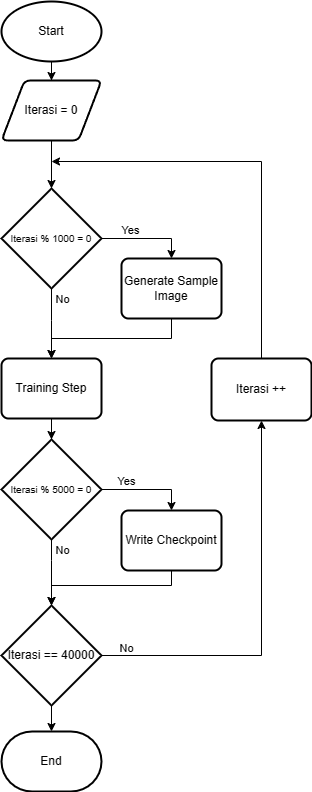
\includegraphics[scale=0.47]{gambar/Training_model.png}
  \caption{Diagram Proses Training Model Keseluruhan}
  \label{fig:training}
\end{figure}

Untuk setiap 1 iterasi proses training, model akan menjalankan proses yang alurnya dapat dilihat pada gambar \ref{fig:arsitekturGAN}. 
Gambar Input akan dimasukkan ke Generator, dan akan menghasilkan Gambar sintesis. 
Discriminator akan memproses 2 pasangan input, yaitu pasangan gambar input dengan gambar asli, dan pasangan gambar input dengan gambar sintesis. 
Pada pasangan pertama, akan diperoleh output Discriminator dari gambar asli, dan pasangan kedua akan diperoleh output Discriminator dari gambar sintesis. 

Generator Loss akan memproses output Discriminator dari gambar sintesis, bersama dengan gambar hasil sintesis dan gambar asli. 
Hasil dari Total Generator Loss akan diterima oleh Generator Optimizer, dan akan diterapkan ke Generator di iterasi berikutnya. 
Discriminator Loss akan memproses output Discriminator dari gambar sintesis dan dari gambar asli. 
Hasil dari Total Discriminator Loss akan diterima oleh Discriminator Optimizer, dan akan diterapkan ke Discriminator di iterasi berikutnya.

\subsection{Evaluasi Model}
\label{subsec:evaluasi}

Setelah model mengalami proses training, model akan dites dengan menggunakan test data. 
Test data berupa 40 data dari dataset yang belum dilatih pada model. 
\emph{Checkpoint} yang disimpan terakhir akan dimuat, dan akan dicoba untuk mensintesis gambar menggunakan test data tersebut. 

Proses evaluasi dilakukan dengan evaluasi matriks kemudian dilanjut dengan evaluasi visual. 
Evaluasi matriks adalah metode objektif yang menggunakan berbagai metrik dan parameter numerik untuk mengukur sejauh mana dua gambar cocok atau berbeda. 
Metode evaluasi matriks yang digunakan pada penelitian ini adalah metode \emph{Root Mean Square} (RMS), \emph{Mean Square Error} (MSE) dan \emph{Structural Similarity Index} (SSIM). 
RMS dan MSE umumnya digunakan untuk mengukur kesalahan atau perbedaan antara dua gambar atau sinyal, dengan nilai yang lebih rendah menunjukkan kesamaan yang lebih besar. 
Sedangkan SSIM memberikan ukuran yang lebih holistik tentang kesamaan struktural antara dua gambar.

Setelah melakukan evaluasi matriks, dilakukan evaluasi visual. 
Evaluasi visual dilakukan dengan melibatkan penilaian subjektif oleh manusia terhadap kualitas dan kemiripan dua gambar. 
Dalam membantu proses evaluasi visual, digunakan fungsi \emph{image differencing}. 
Fungsi \emph{image differencing} melibatkan pengurangan piksel-piksel dari gambar asli dengan gambar sintesis. 
Hasil pengurangan dapat mengungkapkan informasi penting tentang perubahan struktur, pergeseran objek, atau perubahan lainnya dalam gambar.

\section{Bahan dan Peralatan yang Digunakan}
\label{sec:bahanPeralatan}

\subsection{GprMax}
\label{subsec:GprMax}

GprMax merupakan perangkat lunak open source yang mensimulasikan perambatan gelombang elektromagnetik. 
GprMax menggunakan metode Finite Difference Time-Domain (FDTD) dalam pemodelan numerik sinyal GPR. 
Kode pada gprMax aslinya berbasis C, dan sekarang sudah sepenuhnya ditulis ulang menggunakan kombinasi bahasa Python dan Cython. 
GprMax menggunakan file berbasis teks di mana setiap parameter simulasi ditentukan oleh pengguna. 
Parameter tersebut antara lain ukuran model, diskritasi, waktu simulasi, bentuk geometri, material, dan eksitasi.

\subsection{Paraview}
\label{paraview}

Paraview merupakan suatu aplikasi untuk memvisualisasikan dan menganalisis kumpulan data yang sangat besar.
Aplikasi ini menyediakan \emph{Graphical User Interface} (GUI) untuk pembuatan dan pelaksanaan visualisasi secara dinamis.
ParaView mendukung visualisasi dan rendering kumpulan data besar dengan menjalankan program ini secara paralel pada mesin memori bersama atau terdistribusi. 
ParaView mendukung \emph{hardware-accelerated parallel rendering} dan mencapai kinerja \emph{rendering} yang interaktif melalui teknik \emph{level-of-detail}.
Desain menyeimbangkan dan mengintegrasikan sejumlah persyaratan yang beragam termasuk kemampuan untuk menangani data besar, kemudahan penggunaan, dan ekstensibilitas oleh pengembang \parencite{paraview}.

\subsection{Jupyter Notebook}
\label{subsec:jupyter}

Jupyter Notebook merupakan aplikasi web untuk membuat dan membagikan dokumen. 
Dokumen biasa berisi kode, persamaan matematika, visualisasi gambar, maupun teks. 
Jupyter Notebook disajikan dalam bentuk kernel IPython, sehingga memungkinkan pengguna untuk menulis program dengan bahasa Python. 
Pada gprMax, Jupyter Notebook merupakan salah satu tools yang dapat digunakan dalam memplot sinyal GPR.

\subsection{Laptop}
\label{subsec:laptop}

Pada penelitian ini, alat utama yang akan digunakan adalah Laptop Asus TUF Gaming A15 FA506QM dengan Processor AMD Ryzen 7 @ 3.20Ghz, 
Ram 32 GB, 1 TB SSD, NVIDIA Geforce RTX 3060 dan AMD Radeon ™ Graphics Card, serta Sistem Operasi Windows.

\cleardoublepage

% Bab 4 pengujian dan analisis
\chapter{HASIL DAN PEMBAHASAN}
\label{chap:hasilpembahasan}

\section{Simulasi Dataset GPR}
\label{sec:simulasiDatasetGPR}

Penelitian ini menggunakan dataset GPR buatan sendiri dari hasil simulasi gprMax. 
Simulasi gprMax dilakukan untuk mendapat 2 jenis data, yaitu data gambar \emph{B-scan} GPR dan data gambar bentuk geometri simulasi. 
Untuk data gambar \emph{B-scan} membutuhkan waktu sekitar 15-20 menit per simulasi, sedangkan untuk data gambar bentuk geometri simulasi membutuhkan waktu sekitar 5-10 menit per simulasi. 
Sehingga total waktu yang dibutuhkan untuk mensimulasikan 200 dari data gambar \emph{B-scan} GPR dan data gambar bentuk geometri simulasi serta penggabungan kedua data menjadi satu sekitar 85 jam.

Dari 200 data GPR, 160 data digunakan untuk proses pelatihan model dan 40 data untuk proses evaluasi model. 
Parameter simulasi pada data ini dibuat acak dengan batasan tertentu untuk data pelatihan dan dibuat menyesuaikan variasi untuk data test. 
Dataset penelitian divariasikan berdasarkan kategori sebagai berikut.

\begin{enumerate}[nolistsep]

  \item Objek berbentuk regular

  \item Kompleksitas bentuk objek

  \item Ukuran objek
  
  \item Posisi objek di bawah permukaan

\end{enumerate}

Pada kategori variasi objek berbentuk regular, data dibedakan berdasar bentuk reguler objek, yaitu data dengan objek berbentuk lingkaran (silinder tampak depan) dan data dengan objek berbentuk segi empat (silinder tampak samping). 
Objek hanya terdiri dari 1 objek penyusun, dengan posisi dan ukuran yang dibebaskan, yaitu posisi sekitar 2.5-10 cm di bawah permukaan dan ukuran sekitar 3-10 cm. 
Contoh data untuk variasi ini dapat dilihat pada gambar \ref{fig:regularData}.

\begin{figure}[ht]
  \centering
  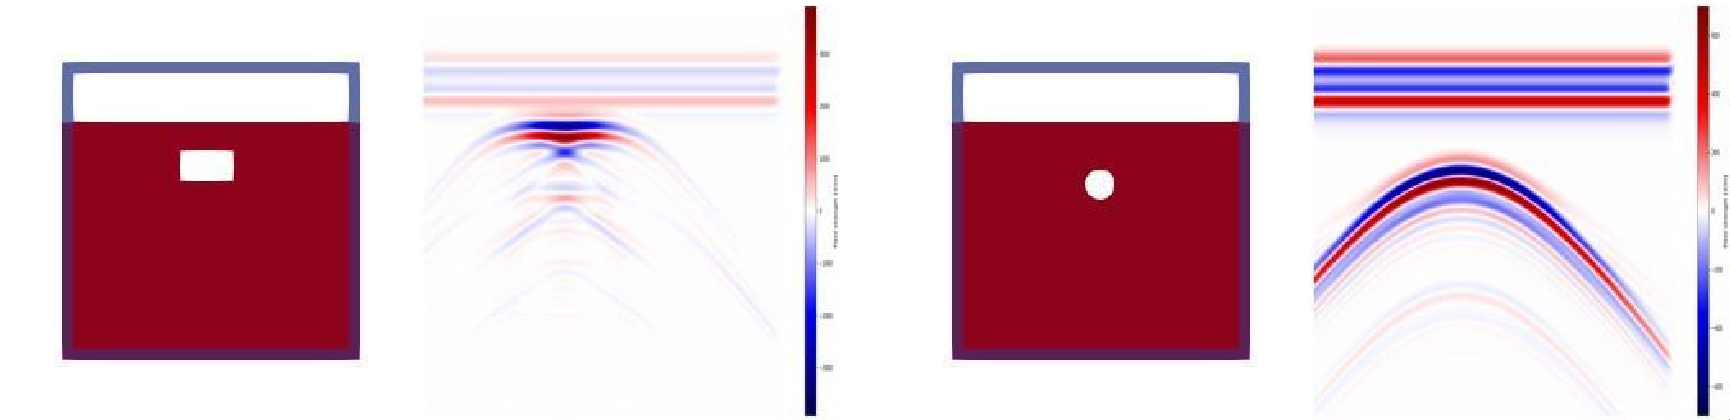
\includegraphics[scale=0.4]{gambar/variasi reguler.png}
  \caption{Data dengan Objek Berbentuk Lingkaran (Kanan) dan Data dengan Objek Berbentuk Segi Empat (Kiri)}
  \label{fig:regularData}
\end{figure}

Pada kategori variasi kompleksitas bentuk objek, data dibedakan berdasar banyak objek penyusun yang digabung, yaitu data dengan objek sederhana dan data dengan objek kompleks. 
Objek sederhana memiliki sekitar 3-6 objek penyusun, sedangkan objek kompleks memiliki sekitar 10-15 objek penyusun. 
Posisi objek dan ukuran objek penyusun kedua data disamakan, yaitu posisi sekitar 6.5 cm di bawah permukaan dan ukuran objek penyusun sekitar 1.5 cm. 
Contoh data untuk variasi ini dapat dilihat pada gambar \ref{fig:kompleksData}.

\begin{figure}[ht]
  \centering
  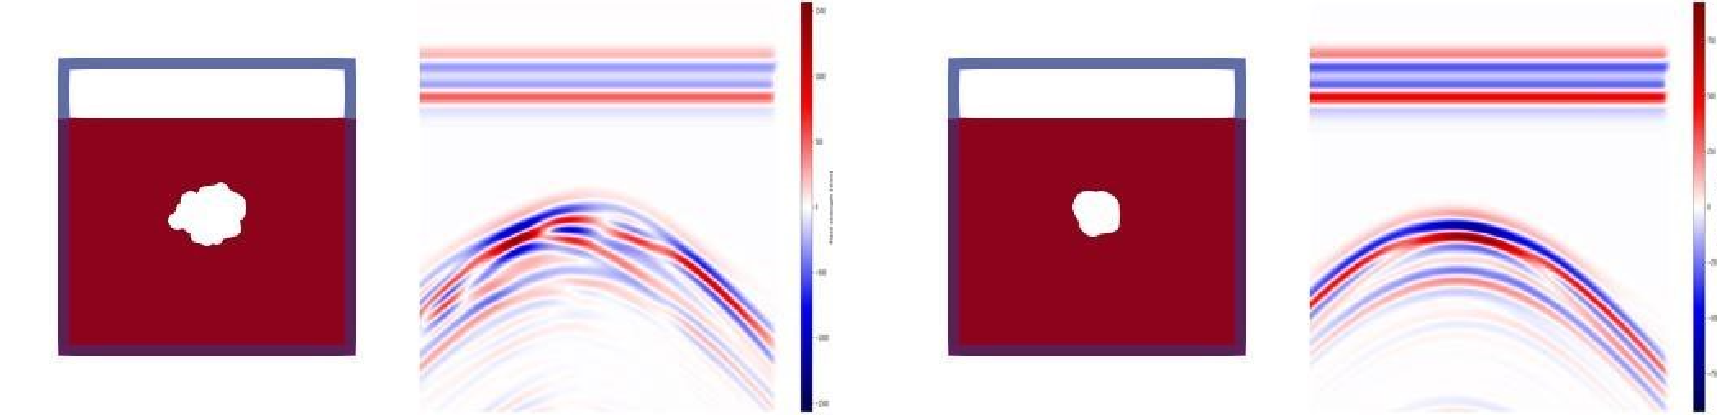
\includegraphics[scale=0.4]{gambar/variasi kompleksitas.png}
  \caption{Data dengan Objek Berbentuk Sederhana (Kanan) dan Data dengan Objek Berbentuk Kompleks (Kiri)}
  \label{fig:kompleksData}
\end{figure}

Pada kategori variasi ukuran objek, data dibedakan berdasar besar ukuran objek, yaitu data dengan objek kecil dan data dengan objek besar. 
Objek kecil memiliki ukuran sekitar 3-4 cm, sedangkan objek besar memiliki ukuran sekitar 5-6 cm. 
Jumlah objek penyusun serta posisi objek disamakan, yaitu objek penyusun sejumlah 5 buah dan kedalaman sekitar 4.5 cm. 
Contoh data untuk variasi ini dapat dilihat pada gambar \ref{fig:ukuranData}.

\begin{figure}[ht]
  \centering
  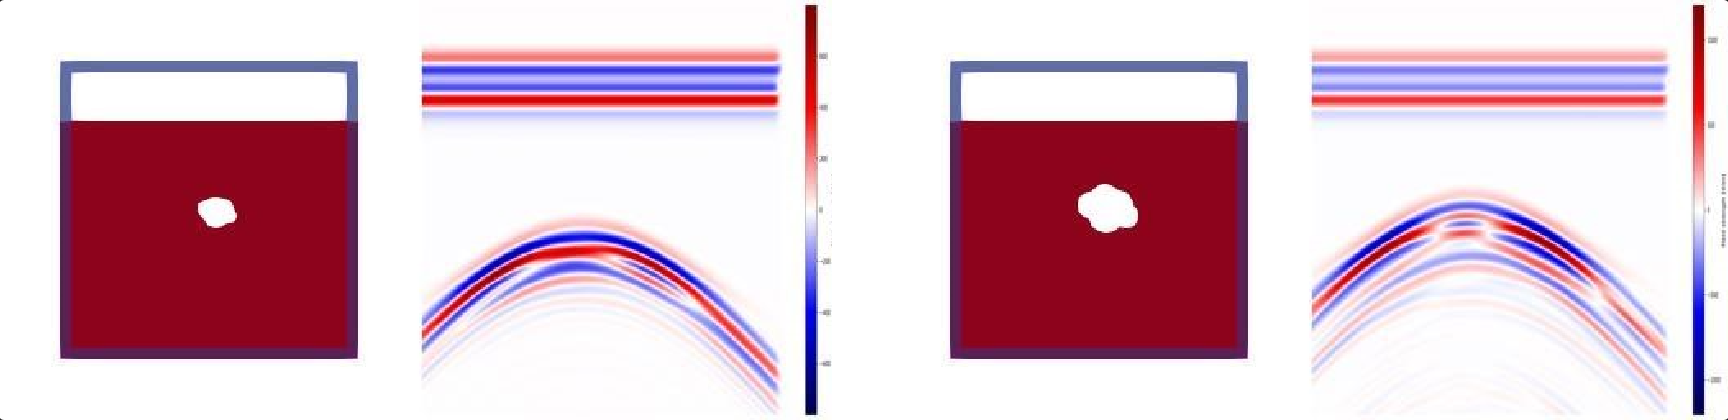
\includegraphics[scale=0.4]{gambar/variasi ukuran.png}
  \caption{Data dengan Objek Berukuran Besar (Kanan) dan Data dengan Objek Berukuran Kecil (Kiri)}
  \label{fig:ukuranData}
\end{figure}

Pada kategori variasi Posisi objek di bawah permukaan, data dibedakan berdasar posisi objek dari permukaan, yaitu data dengan objek dangkal dan data dengan objek dalam. 
Objek dangkal memiliki posisi sekitar 2.5 cm dari permukaan, sedangkan objek dalam memiliki posisi sekitar 7.5 cm dari permukaan. 
Ukuran objek dan jumlah objek penyusun disamakan, yaitu ukuran objek sekitar 4.5 cm dan jumlah objek penyusun sejumlah 5 buah. 
Contoh data untuk variasi ini dapat dilihat pada gambar \ref{fig:posisiData}.

\begin{figure}[ht]
  \centering
  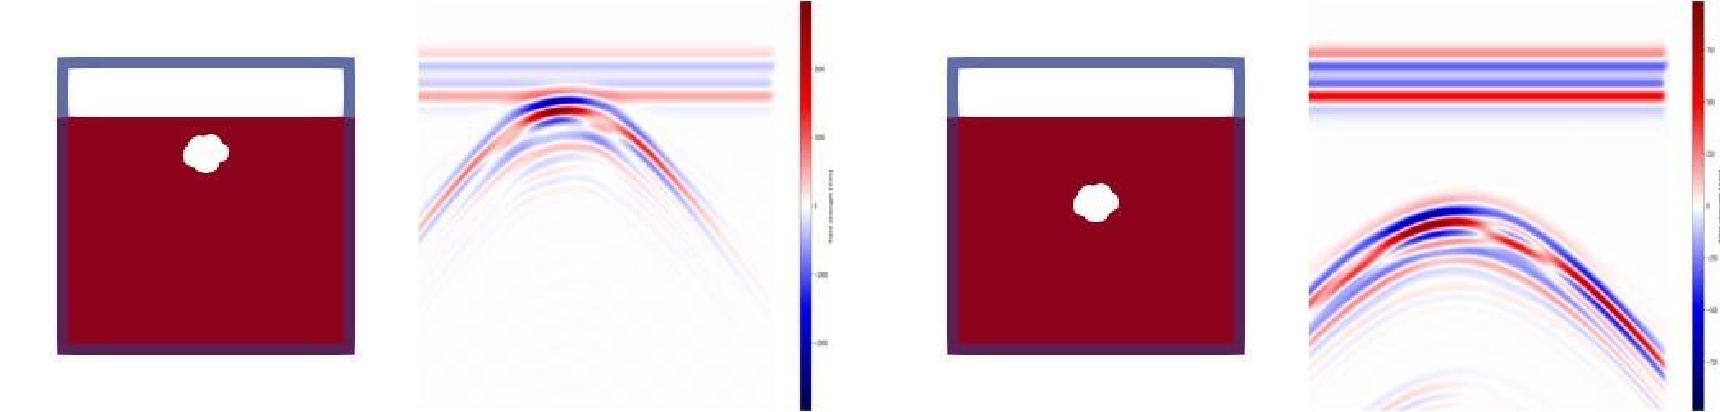
\includegraphics[scale=0.4]{gambar/variasi kedalaman.png}
  \caption{Data dengan Posisi Objek Jauh dari Permukaan (Kanan) dan Data dengan Posisi Objek Dekat dari Permukaan (Kiri)}
  \label{fig:posisiData}
\end{figure}

\section{Hasil Pelatihan Model GAN}
\label{sec:hasilpelatihanGAN}

Proses pelatihan model dilakukan sebanyak 40.000 iterasi. 
Total waktu yang diperlukan untuk menjalankan keseluruhan proses pelatihan selama 9 jam mulai jam 20.00 WIB hingga pukul 05.00 WIB esok harinya. 
Selama pelatihan, nilai \emph{total discriminator loss} dan \emph{total generator loss} disimpan ke sebuah \emph{log}. 
Dengan menggunakan tensorboard, nilai \emph{loss} yang disimpan pada \emph{log} dapat divisualisasikan dalam bentuk grafik. 

\begin{figure}[ht]
  \centering
  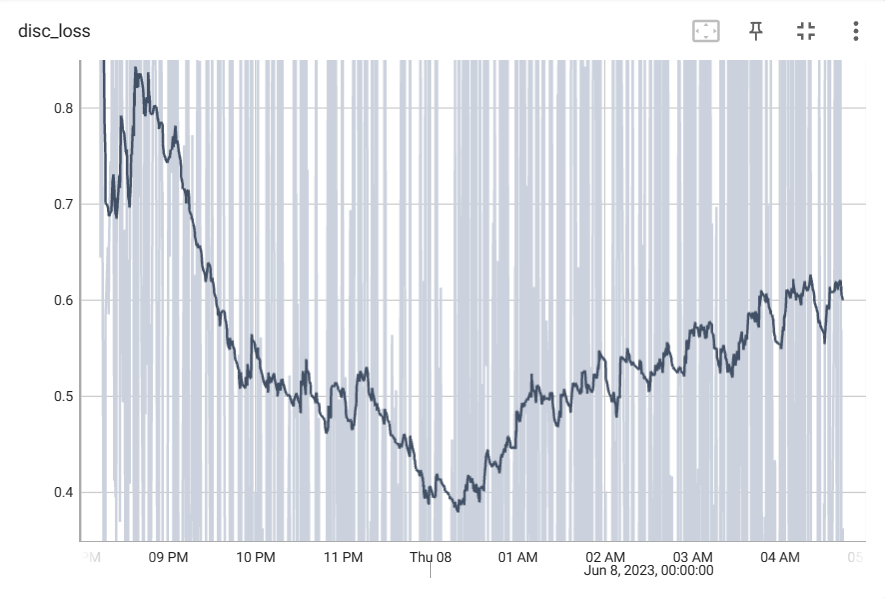
\includegraphics[scale=0.6]{gambar/Disc_loss.png}
  \caption{Grafik Total Discriminator Loss}
  \label{fig:discLoss}
\end{figure}

Gambar \ref{fig:discLoss} menunjukkan grafik \emph{discriminator loss} yang awalnya semakin mengecil kemudian mengalami peningkatan. 
Hal ini menunjukkan bahwa discriminator awalnya semakin baik dalam mempelajari perbedaan data asli dengan data yang disintesis. 
Setelah melewati waktu tertentu, discriminator kemudian menjadi semakin sulit dalam mempelajari perbedaan tersebut. 

\begin{figure}[ht]
  \centering
  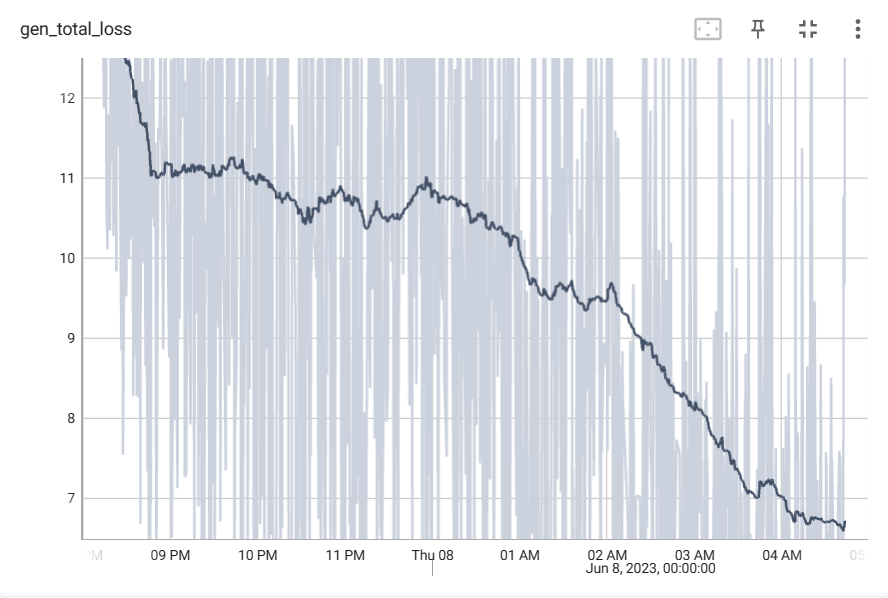
\includegraphics[scale=0.6]{gambar/Gen_total_loss.png}
  \caption{Grafik Total Generator Loss}
  \label{fig:genLoss}
\end{figure}

Gambar \ref{fig:genLoss} menunjukkan grafik \emph{generator loss} yang semakin lama semakin mengecil. 
Hal ini menunjukkan bahwa generator semakin baik dalam mempelajari dan menghasilkan data sintesis yang sesuai dengan data asli. 
Grafik juga menunjukkan penurunan nilai yang lumayan konstan, sehingga dapat dikatakan model generator dilatih secara baik pada proses pelatihan model GAN.

Dalam proses pelatihan model GAN, penting untuk membandingkan nilai atau grafik \emph{generator loss} dan \emph{discriminator loss}. 
Pada kedua grafik, dapat dilihat bahwa awalnya perubahan kedua nilai \emph{loss} sama-sama menurun, yang menunjukkan proses model dalam mempelajari data berjalan dengan baik. 
Namun, sekitar pukul 00.00 grafik dari \emph{discriminator loss} menjadi semakin meningkat, sedangkan grafik \emph{generator loss} tetap semakin menurun. 
Hal ini menunjukkan bahwa pada interval waktu tersebut, discriminator sudah mulai kesulitan dalam membedakan gambar asli dengan gambar palsu, sedangkan generator tetap semakin baik dalam menghasilkan output yang sesuai dengan aslinya.

\section{Hasil Evaluasi Output GAN}
\label{sec:evaluasiOutput}

Data penelitian menggunakan 200 data hasil simulasi gprMax untuk gambar \emph{B-scan} GPR beserta bentuk geometri dari simulasi. 
Dari 200 total data, 40 data digunakan sebagai test data dan dilakukan evaluasi model GAN. 
Proses evaluasi dilakukan dengan evaluasi matriks kemudian dilanjut dengan evaluasi visual. 
Evaluasi matriks dilakukan dengan menggunakan 3 metode, yaitu metode RMS, MSE, dan SSIM. 
Untuk nilai hasil RMS dan MSE dikatakan baik jika nilainya semakin mendekati 0, sedangkan untuk nilai hasil SSIM dikatakan baik jika nilainya semakin mendekati 1. 
Hasil dari evaluasi matriks untuk keseluruhan data dapat dilihat pada tabel \ref{tb:evaluasimatriks}. 

\begin{table}[]
  \caption{Tabel Nilai RMS, MSE dan SSIM dari Gambar Sintesis dengan Gambar Asli Setiap Variasi Data}
  \label{tb:evaluasimatriks}
  \begin{tabular}{|l|cc|cc|cc|}
  \hline
  \multicolumn{1}{|c|}{Variasi Data}                  & \multicolumn{2}{c|}{RMS}                                                                               & \multicolumn{2}{c|}{MSE}                                                                                   & \multicolumn{2}{c|}{SSIM}                                                                            \\ \hline
                                                      & \multicolumn{1}{c|}{\cellcolor[HTML]{FFFFFF}24.343} & \cellcolor[HTML]{FFFFFF}                         & \multicolumn{1}{c|}{\cellcolor[HTML]{FFFFFF}849.059}  & \cellcolor[HTML]{FFFFFF}                           & \multicolumn{1}{c|}{\cellcolor[HTML]{FFFFFF}0.861} & \cellcolor[HTML]{FFFFFF}                        \\ \cline{2-2} \cline{4-4} \cline{6-6}
                                                      & \multicolumn{1}{c|}{\cellcolor[HTML]{FFFFFF}23.515} & \cellcolor[HTML]{FFFFFF}                         & \multicolumn{1}{c|}{\cellcolor[HTML]{FFFFFF}925.548}  & \cellcolor[HTML]{FFFFFF}                           & \multicolumn{1}{c|}{\cellcolor[HTML]{FFFFFF}0.845} & \cellcolor[HTML]{FFFFFF}                        \\ \cline{2-2} \cline{4-4} \cline{6-6}
                                                      & \multicolumn{1}{c|}{\cellcolor[HTML]{FFFFFF}26.168} & \cellcolor[HTML]{FFFFFF}                         & \multicolumn{1}{c|}{\cellcolor[HTML]{FFFFFF}1232.388} & \cellcolor[HTML]{FFFFFF}                           & \multicolumn{1}{c|}{\cellcolor[HTML]{FFFFFF}0.826} & \cellcolor[HTML]{FFFFFF}                        \\ \cline{2-2} \cline{4-4} \cline{6-6}
                                                      & \multicolumn{1}{c|}{\cellcolor[HTML]{FFFFFF}24.361} & \cellcolor[HTML]{FFFFFF}                         & \multicolumn{1}{c|}{\cellcolor[HTML]{FFFFFF}1047.606} & \cellcolor[HTML]{FFFFFF}                           & \multicolumn{1}{c|}{\cellcolor[HTML]{FFFFFF}0.841} & \cellcolor[HTML]{FFFFFF}                        \\ \cline{2-2} \cline{4-4} \cline{6-6}
  \multirow{-5}{*}{Bentuk Regular Lingkaran}          & \multicolumn{1}{c|}{\cellcolor[HTML]{FFFFFF}24.048} & \multirow{-5}{*}{\cellcolor[HTML]{FFFFFF}24.487} & \multicolumn{1}{c|}{\cellcolor[HTML]{FFFFFF}1056.576} & \multirow{-5}{*}{\cellcolor[HTML]{FFFFFF}1022.235} & \multicolumn{1}{c|}{\cellcolor[HTML]{FFFFFF}0.843} & \multirow{-5}{*}{\cellcolor[HTML]{FFFFFF}0.843} \\ \hline
                                                      & \multicolumn{1}{c|}{26.549}                         & \cellcolor[HTML]{FFFFFF}                         & \multicolumn{1}{c|}{1160.144}                         & \cellcolor[HTML]{FFFFFF}                           & \multicolumn{1}{c|}{0.843}                         & \cellcolor[HTML]{FFFFFF}                        \\ \cline{2-2} \cline{4-4} \cline{6-6}
                                                      & \multicolumn{1}{l|}{28.027}                         & \cellcolor[HTML]{FFFFFF}                         & \multicolumn{1}{l|}{1060.923}                         & \cellcolor[HTML]{FFFFFF}                           & \multicolumn{1}{l|}{0.849}                         & \cellcolor[HTML]{FFFFFF}                        \\ \cline{2-2} \cline{4-4} \cline{6-6}
                                                      & \multicolumn{1}{l|}{24.116}                         & \cellcolor[HTML]{FFFFFF}                         & \multicolumn{1}{l|}{919.714}                          & \cellcolor[HTML]{FFFFFF}                           & \multicolumn{1}{l|}{0.857}                         & \cellcolor[HTML]{FFFFFF}                        \\ \cline{2-2} \cline{4-4} \cline{6-6}
                                                      & \multicolumn{1}{l|}{27.656}                         & \cellcolor[HTML]{FFFFFF}                         & \multicolumn{1}{l|}{1266.811}                         & \cellcolor[HTML]{FFFFFF}                           & \multicolumn{1}{l|}{0.833}                         & \cellcolor[HTML]{FFFFFF}                        \\ \cline{2-2} \cline{4-4} \cline{6-6}
  \multirow{-5}{*}{Bentuk Regular Segi Empat}         & \multicolumn{1}{l|}{30.177}                         & \multirow{-5}{*}{\cellcolor[HTML]{FFFFFF}27.305} & \multicolumn{1}{l|}{1395.066}                         & \multirow{-5}{*}{\cellcolor[HTML]{FFFFFF}1160.532} & \multicolumn{1}{l|}{0.809}                         & \multirow{-5}{*}{\cellcolor[HTML]{FFFFFF}0.838} \\ \hline
                                                      & \multicolumn{1}{c|}{\cellcolor[HTML]{FFFFFF}28.446} & \cellcolor[HTML]{FFFFFF}                         & \multicolumn{1}{c|}{\cellcolor[HTML]{FFFFFF}1416.187} & \cellcolor[HTML]{FFFFFF}                           & \multicolumn{1}{c|}{\cellcolor[HTML]{FFFFFF}0.848} & \cellcolor[HTML]{FFFFFF}                        \\ \cline{2-2} \cline{4-4} \cline{6-6}
                                                      & \multicolumn{1}{c|}{\cellcolor[HTML]{FFFFFF}30.685} & \cellcolor[HTML]{FFFFFF}                         & \multicolumn{1}{c|}{\cellcolor[HTML]{FFFFFF}1753.308} & \cellcolor[HTML]{FFFFFF}                           & \multicolumn{1}{c|}{\cellcolor[HTML]{FFFFFF}0.811} & \cellcolor[HTML]{FFFFFF}                        \\ \cline{2-2} \cline{4-4} \cline{6-6}
                                                      & \multicolumn{1}{c|}{\cellcolor[HTML]{FFFFFF}29.959} & \cellcolor[HTML]{FFFFFF}                         & \multicolumn{1}{c|}{\cellcolor[HTML]{FFFFFF}1658.955} & \cellcolor[HTML]{FFFFFF}                           & \multicolumn{1}{c|}{\cellcolor[HTML]{FFFFFF}0.833} & \cellcolor[HTML]{FFFFFF}                        \\ \cline{2-2} \cline{4-4} \cline{6-6}
                                                      & \multicolumn{1}{c|}{\cellcolor[HTML]{FFFFFF}25.723} & \cellcolor[HTML]{FFFFFF}                         & \multicolumn{1}{c|}{\cellcolor[HTML]{FFFFFF}1341.356} & \cellcolor[HTML]{FFFFFF}                           & \multicolumn{1}{c|}{\cellcolor[HTML]{FFFFFF}0.837} & \cellcolor[HTML]{FFFFFF}                        \\ \cline{2-2} \cline{4-4} \cline{6-6}
  \multirow{-5}{*}{Bentuk Objek Sederhana}            & \multicolumn{1}{c|}{\cellcolor[HTML]{FFFFFF}26.653} & \multirow{-5}{*}{\cellcolor[HTML]{FFFFFF}28.293} & \multicolumn{1}{c|}{\cellcolor[HTML]{FFFFFF}1469.097} & \multirow{-5}{*}{\cellcolor[HTML]{FFFFFF}1527.781} & \multicolumn{1}{c|}{\cellcolor[HTML]{FFFFFF}0.816} & \multirow{-5}{*}{\cellcolor[HTML]{FFFFFF}0.829} \\ \hline
                                                      & \multicolumn{1}{c|}{\cellcolor[HTML]{FFFFFF}25.317} & \cellcolor[HTML]{FFFFFF}                         & \multicolumn{1}{c|}{\cellcolor[HTML]{FFFFFF}1368.814} & \cellcolor[HTML]{FFFFFF}                           & \multicolumn{1}{c|}{\cellcolor[HTML]{FFFFFF}0.841} & \cellcolor[HTML]{FFFFFF}                        \\ \cline{2-2} \cline{4-4} \cline{6-6}
                                                      & \multicolumn{1}{c|}{\cellcolor[HTML]{FFFFFF}28.214} & \cellcolor[HTML]{FFFFFF}                         & \multicolumn{1}{c|}{\cellcolor[HTML]{FFFFFF}1611.368} & \cellcolor[HTML]{FFFFFF}                           & \multicolumn{1}{c|}{\cellcolor[HTML]{FFFFFF}0.830} & \cellcolor[HTML]{FFFFFF}                        \\ \cline{2-2} \cline{4-4} \cline{6-6}
                                                      & \multicolumn{1}{c|}{\cellcolor[HTML]{FFFFFF}31.084} & \cellcolor[HTML]{FFFFFF}                         & \multicolumn{1}{c|}{\cellcolor[HTML]{FFFFFF}1970.674} & \cellcolor[HTML]{FFFFFF}                           & \multicolumn{1}{c|}{\cellcolor[HTML]{FFFFFF}0.832} & \cellcolor[HTML]{FFFFFF}                        \\ \cline{2-2} \cline{4-4} \cline{6-6}
                                                      & \multicolumn{1}{c|}{\cellcolor[HTML]{FFFFFF}32.412} & \cellcolor[HTML]{FFFFFF}                         & \multicolumn{1}{c|}{\cellcolor[HTML]{FFFFFF}2002.734} & \cellcolor[HTML]{FFFFFF}                           & \multicolumn{1}{c|}{\cellcolor[HTML]{FFFFFF}0.837} & \cellcolor[HTML]{FFFFFF}                        \\ \cline{2-2} \cline{4-4} \cline{6-6}
  \multirow{-5}{*}{Bentuk Objek Kompleks}             & \multicolumn{1}{c|}{\cellcolor[HTML]{FFFFFF}30.085} & \multirow{-5}{*}{\cellcolor[HTML]{FFFFFF}29.422} & \multicolumn{1}{c|}{\cellcolor[HTML]{FFFFFF}1954.447} & \multirow{-5}{*}{\cellcolor[HTML]{FFFFFF}1781.607} & \multicolumn{1}{c|}{\cellcolor[HTML]{FFFFFF}0.821} & \multirow{-5}{*}{\cellcolor[HTML]{FFFFFF}0.832} \\ \hline
                                                      & \multicolumn{1}{c|}{\cellcolor[HTML]{FFFFFF}34.674} & \cellcolor[HTML]{FFFFFF}                         & \multicolumn{1}{c|}{\cellcolor[HTML]{FFFFFF}1933.112} & \cellcolor[HTML]{FFFFFF}                           & \multicolumn{1}{c|}{\cellcolor[HTML]{FFFFFF}0.799} & \cellcolor[HTML]{FFFFFF}                        \\ \cline{2-2} \cline{4-4} \cline{6-6}
                                                      & \multicolumn{1}{c|}{\cellcolor[HTML]{FFFFFF}23.165} & \cellcolor[HTML]{FFFFFF}                         & \multicolumn{1}{c|}{\cellcolor[HTML]{FFFFFF}919.539}  & \cellcolor[HTML]{FFFFFF}                           & \multicolumn{1}{c|}{\cellcolor[HTML]{FFFFFF}0.831} & \cellcolor[HTML]{FFFFFF}                        \\ \cline{2-2} \cline{4-4} \cline{6-6}
                                                      & \multicolumn{1}{c|}{\cellcolor[HTML]{FFFFFF}28.873} & \cellcolor[HTML]{FFFFFF}                         & \multicolumn{1}{c|}{\cellcolor[HTML]{FFFFFF}1529.034} & \cellcolor[HTML]{FFFFFF}                           & \multicolumn{1}{c|}{\cellcolor[HTML]{FFFFFF}0.829} & \cellcolor[HTML]{FFFFFF}                        \\ \cline{2-2} \cline{4-4} \cline{6-6}
                                                      & \multicolumn{1}{c|}{\cellcolor[HTML]{FFFFFF}21.590} & \cellcolor[HTML]{FFFFFF}                         & \multicolumn{1}{c|}{\cellcolor[HTML]{FFFFFF}872.725}  & \cellcolor[HTML]{FFFFFF}                           & \multicolumn{1}{c|}{\cellcolor[HTML]{FFFFFF}0.857} & \cellcolor[HTML]{FFFFFF}                        \\ \cline{2-2} \cline{4-4} \cline{6-6}
  \multirow{-5}{*}{Ukuran Objek Kecil}                & \multicolumn{1}{c|}{\cellcolor[HTML]{FFFFFF}25.036} & \multirow{-5}{*}{\cellcolor[HTML]{FFFFFF}26.668} & \multicolumn{1}{c|}{\cellcolor[HTML]{FFFFFF}1199.543} & \multirow{-5}{*}{\cellcolor[HTML]{FFFFFF}1290.791} & \multicolumn{1}{c|}{\cellcolor[HTML]{FFFFFF}0.829} & \multirow{-5}{*}{\cellcolor[HTML]{FFFFFF}0.829} \\ \hline
                                                      & \multicolumn{1}{c|}{\cellcolor[HTML]{FFFFFF}27.415} & \cellcolor[HTML]{FFFFFF}                         & \multicolumn{1}{c|}{\cellcolor[HTML]{FFFFFF}1476.994} & \cellcolor[HTML]{FFFFFF}                           & \multicolumn{1}{c|}{\cellcolor[HTML]{FFFFFF}0.818} & \cellcolor[HTML]{FFFFFF}                        \\ \cline{2-2} \cline{4-4} \cline{6-6}
                                                      & \multicolumn{1}{c|}{\cellcolor[HTML]{FFFFFF}35.830} & \cellcolor[HTML]{FFFFFF}                         & \multicolumn{1}{c|}{\cellcolor[HTML]{FFFFFF}2220.673} & \cellcolor[HTML]{FFFFFF}                           & \multicolumn{1}{c|}{\cellcolor[HTML]{FFFFFF}0.817} & \cellcolor[HTML]{FFFFFF}                        \\ \cline{2-2} \cline{4-4} \cline{6-6}
                                                      & \multicolumn{1}{c|}{\cellcolor[HTML]{FFFFFF}28.350} & \cellcolor[HTML]{FFFFFF}                         & \multicolumn{1}{c|}{\cellcolor[HTML]{FFFFFF}1602.741} & \cellcolor[HTML]{FFFFFF}                           & \multicolumn{1}{c|}{\cellcolor[HTML]{FFFFFF}0.825} & \cellcolor[HTML]{FFFFFF}                        \\ \cline{2-2} \cline{4-4} \cline{6-6}
                                                      & \multicolumn{1}{c|}{\cellcolor[HTML]{FFFFFF}27.847} & \cellcolor[HTML]{FFFFFF}                         & \multicolumn{1}{c|}{\cellcolor[HTML]{FFFFFF}1421.890} & \cellcolor[HTML]{FFFFFF}                           & \multicolumn{1}{c|}{\cellcolor[HTML]{FFFFFF}0.833} & \cellcolor[HTML]{FFFFFF}                        \\ \cline{2-2} \cline{4-4} \cline{6-6}
  \multirow{-5}{*}{Ukuran Objek Besar}                & \multicolumn{1}{c|}{\cellcolor[HTML]{FFFFFF}26.131} & \multirow{-5}{*}{\cellcolor[HTML]{FFFFFF}29.115} & \multicolumn{1}{c|}{\cellcolor[HTML]{FFFFFF}1302.681} & \multirow{-5}{*}{\cellcolor[HTML]{FFFFFF}1604.996} & \multicolumn{1}{c|}{\cellcolor[HTML]{FFFFFF}0.826} & \multirow{-5}{*}{\cellcolor[HTML]{FFFFFF}0.824} \\ \hline
                                                      & \multicolumn{1}{c|}{\cellcolor[HTML]{FFFFFF}27.983} & \cellcolor[HTML]{FFFFFF}                         & \multicolumn{1}{c|}{\cellcolor[HTML]{FFFFFF}1259.261} & \cellcolor[HTML]{FFFFFF}                           & \multicolumn{1}{c|}{\cellcolor[HTML]{FFFFFF}0.842} & \cellcolor[HTML]{FFFFFF}                        \\ \cline{2-2} \cline{4-4} \cline{6-6}
                                                      & \multicolumn{1}{c|}{\cellcolor[HTML]{FFFFFF}22.333} & \cellcolor[HTML]{FFFFFF}                         & \multicolumn{1}{c|}{\cellcolor[HTML]{FFFFFF}913.083}  & \cellcolor[HTML]{FFFFFF}                           & \multicolumn{1}{c|}{\cellcolor[HTML]{FFFFFF}0.847} & \cellcolor[HTML]{FFFFFF}                        \\ \cline{2-2} \cline{4-4} \cline{6-6}
                                                      & \multicolumn{1}{c|}{\cellcolor[HTML]{FFFFFF}27.373} & \cellcolor[HTML]{FFFFFF}                         & \multicolumn{1}{c|}{\cellcolor[HTML]{FFFFFF}1353.813} & \cellcolor[HTML]{FFFFFF}                           & \multicolumn{1}{c|}{\cellcolor[HTML]{FFFFFF}0.821} & \cellcolor[HTML]{FFFFFF}                        \\ \cline{2-2} \cline{4-4} \cline{6-6}
                                                      & \multicolumn{1}{c|}{\cellcolor[HTML]{FFFFFF}25.660} & \cellcolor[HTML]{FFFFFF}                         & \multicolumn{1}{c|}{\cellcolor[HTML]{FFFFFF}1173.256} & \cellcolor[HTML]{FFFFFF}                           & \multicolumn{1}{c|}{\cellcolor[HTML]{FFFFFF}0.847} & \cellcolor[HTML]{FFFFFF}                        \\ \cline{2-2} \cline{4-4} \cline{6-6}
  \multirow{-5}{*}{Posisi Objek Dekat dari Permukaan} & \multicolumn{1}{c|}{\cellcolor[HTML]{FFFFFF}26.464} & \multirow{-5}{*}{\cellcolor[HTML]{FFFFFF}25.963} & \multicolumn{1}{c|}{\cellcolor[HTML]{FFFFFF}1078.885} & \multirow{-5}{*}{\cellcolor[HTML]{FFFFFF}1155.660} & \multicolumn{1}{c|}{\cellcolor[HTML]{FFFFFF}0.846} & \multirow{-5}{*}{\cellcolor[HTML]{FFFFFF}0.841} \\ \hline
                                                      & \multicolumn{1}{c|}{\cellcolor[HTML]{FFFFFF}30.246} & \cellcolor[HTML]{FFFFFF}                         & \multicolumn{1}{c|}{\cellcolor[HTML]{FFFFFF}1603.105} & \cellcolor[HTML]{FFFFFF}                           & \multicolumn{1}{c|}{\cellcolor[HTML]{FFFFFF}0.816} & \cellcolor[HTML]{FFFFFF}                        \\ \cline{2-2} \cline{4-4} \cline{6-6}
                                                      & \multicolumn{1}{c|}{\cellcolor[HTML]{FFFFFF}24.919} & \cellcolor[HTML]{FFFFFF}                         & \multicolumn{1}{c|}{\cellcolor[HTML]{FFFFFF}1201.229} & \cellcolor[HTML]{FFFFFF}                           & \multicolumn{1}{c|}{\cellcolor[HTML]{FFFFFF}0.828} & \cellcolor[HTML]{FFFFFF}                        \\ \cline{2-2} \cline{4-4} \cline{6-6}
                                                      & \multicolumn{1}{c|}{\cellcolor[HTML]{FFFFFF}22.354} & \cellcolor[HTML]{FFFFFF}                         & \multicolumn{1}{c|}{\cellcolor[HTML]{FFFFFF}910.400}  & \cellcolor[HTML]{FFFFFF}                           & \multicolumn{1}{c|}{\cellcolor[HTML]{FFFFFF}0.852} & \cellcolor[HTML]{FFFFFF}                        \\ \cline{2-2} \cline{4-4} \cline{6-6}
                                                      & \multicolumn{1}{c|}{\cellcolor[HTML]{FFFFFF}25.499} & \cellcolor[HTML]{FFFFFF}                         & \multicolumn{1}{c|}{\cellcolor[HTML]{FFFFFF}1168.513} & \cellcolor[HTML]{FFFFFF}                           & \multicolumn{1}{c|}{\cellcolor[HTML]{FFFFFF}0.823} & \cellcolor[HTML]{FFFFFF}                        \\ \cline{2-2} \cline{4-4} \cline{6-6}
  \multirow{-5}{*}{Posisi Objek Jauh dari Permukaan}  & \multicolumn{1}{c|}{\cellcolor[HTML]{FFFFFF}27.806} & \multirow{-5}{*}{\cellcolor[HTML]{FFFFFF}26.165} & \multicolumn{1}{c|}{\cellcolor[HTML]{FFFFFF}1454.938} & \multirow{-5}{*}{\cellcolor[HTML]{FFFFFF}1267.637} & \multicolumn{1}{c|}{\cellcolor[HTML]{FFFFFF}0.831} & \multirow{-5}{*}{\cellcolor[HTML]{FFFFFF}0.829} \\ \hline
  Rata-Rata                                           & \multicolumn{2}{c|}{\cellcolor[HTML]{FFFFFF}27.177}                                                    & \multicolumn{2}{c|}{1351.405}                                                                              & \multicolumn{2}{c|}{0.833}                                                                           \\ \hline
  \end{tabular}
\end{table}

Setelah melakukan evaluasi matriks, dilakukan evaluasi visual. 
Evaluasi visual dilakukan dengan menggunakan fungsi differential map, yang mengurangkan piksel-piksel dari gambar asli dengan gambar sintesis. 
Hasil evaluasi visual akan ditampilkan dengan gambar, dimana semakin gelap (hitam) warna suatu daerah gambar tertentu, maka semakin identik gambar asli dengan gambar sintesis. 
Sebaliknya, semakin terang (putih) warna suatu daerah gambar tertentu, maka semakin berbeda gambar asli dengan gambar sintesis.

Pada variasi objek berbentuk regular, terlihat untuk objek berbentuk lingkaran memiliki rata-rata nilai evaluasi matriks yang lebih baik dari objek berbentuk segi empat. 
Perbedaan rata-rata evaluasi matriks terlihat cukup jauh di antara kedua variasi data. 
Namun, untuk beberapa data terdapat beberapa anomali, seperti data ketiga dari variasi objek lingkaran dan data kedua dari objek segi empat. 

\begin{figure}[ht]
  \centering
  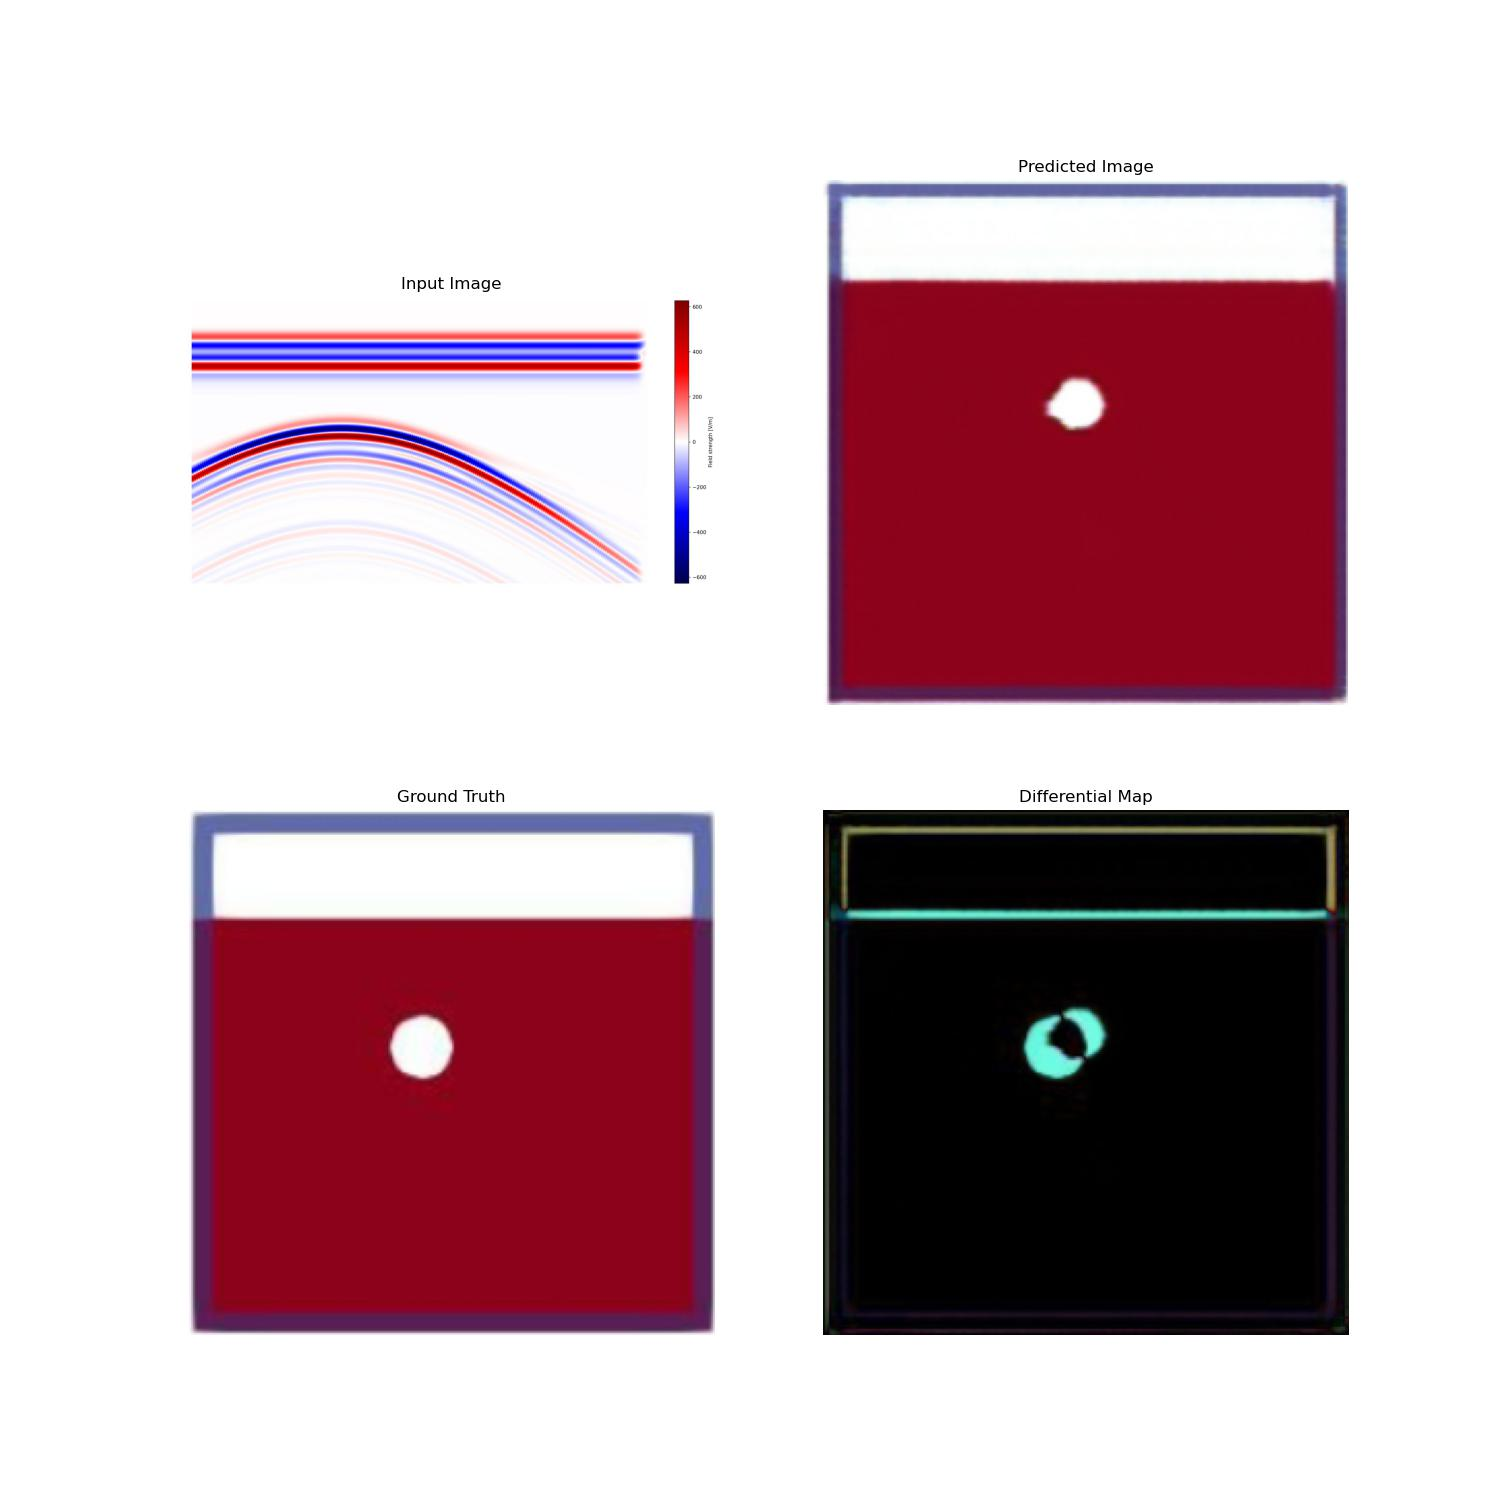
\includegraphics[scale=0.15]{gambar/diffMapLingkaran.jpg}
  \caption{Evaluasi Visual Data Variasi Bentuk Regular Lingkaran}
  \label{fig:diffmaplingkaran}
\end{figure}

Data ketiga dari variasi objek lingkaran memiliki nilai evaluasi matriks yang cukup buruk dari data lain dari variasi yang sama. 
Evaluasi visual dari data dapat dilihat dari gambar \ref{fig:diffmaplingkaran}. 
Pada gambar evaluasi visual dapat dilihat bahwa irisan dari objek sintesis dengan objek asli cukup sedikit sehingga memiliki area error yang cukup luas. 
Hal ini menunjukkan bahwa posisi benda belum sepenuhnya dapat dideteksi oleh model.

\begin{figure}[ht]
  \centering
  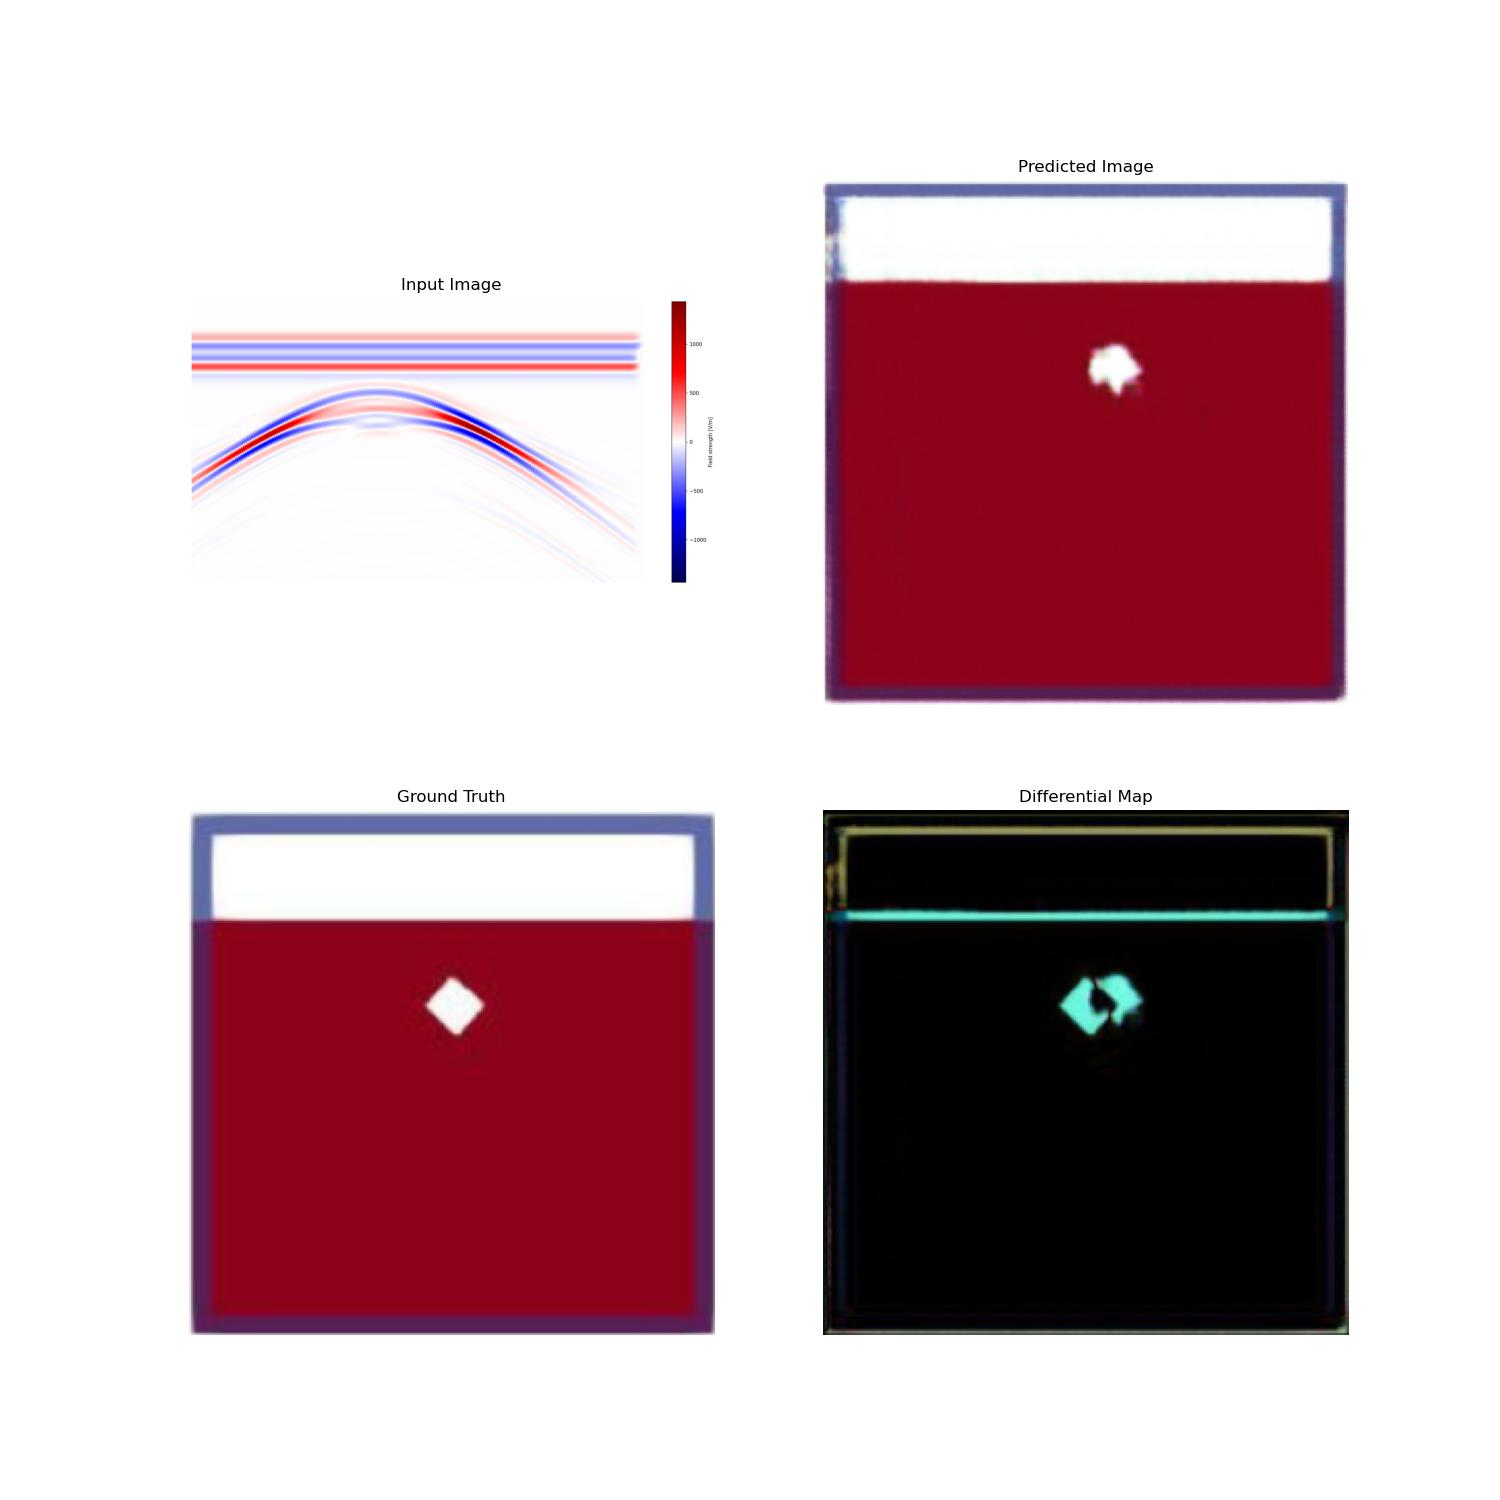
\includegraphics[scale=0.15]{gambar/diffMapSegi4.jpg}
  \caption{Evaluasi Visual Data Variasi Bentuk Regular Segi Empat}
  \label{fig:diffmapsegi4}
\end{figure}

Data kedua dari variasi objek segi empat memiliki nilai evaluasi matriks yang cukup baik dari data lain dari variasi yang sama. 
Evaluasi visual dari data dapat dilihat dari gambar \ref{fig:diffmapsegi4}. 
Pada gambar evaluasi visual dapat dilihat bahwa tidak ada irisan dari gambar sintesis dengan gambar asli, bahkan gambar sintesis hampir tidak memiliki bentuk. 
Hal ini menunjukkan bahwa model masih belum bisa mensintesis gambar dari objek regular berbentuk persegi, yang disebabkan oleh kurangnya data yang dipelajari ketika proses training model.

Pada variasi kompleksitas bentuk objek, terlihat untuk objek berbentuk sederhana memiliki rata-rata nilai evaluasi matriks yang lebih baik dari objek berbentuk kompleks. 
Perbedaan rata-rata evaluasi matriks terlihat cukup dekat di antara kedua variasi data.  
Nilai rata-rata SSIM data objek sederhana yang lebih kecil dari nilai rata-rata SSIM data objek kompleks. 
Namun, nilai rata-rata RMS dan MSE data objek sederhana lebih kecil dari nilai rata-rata RMS dan MSE data objek kompleks. 

\begin{figure}[ht]
  \centering
  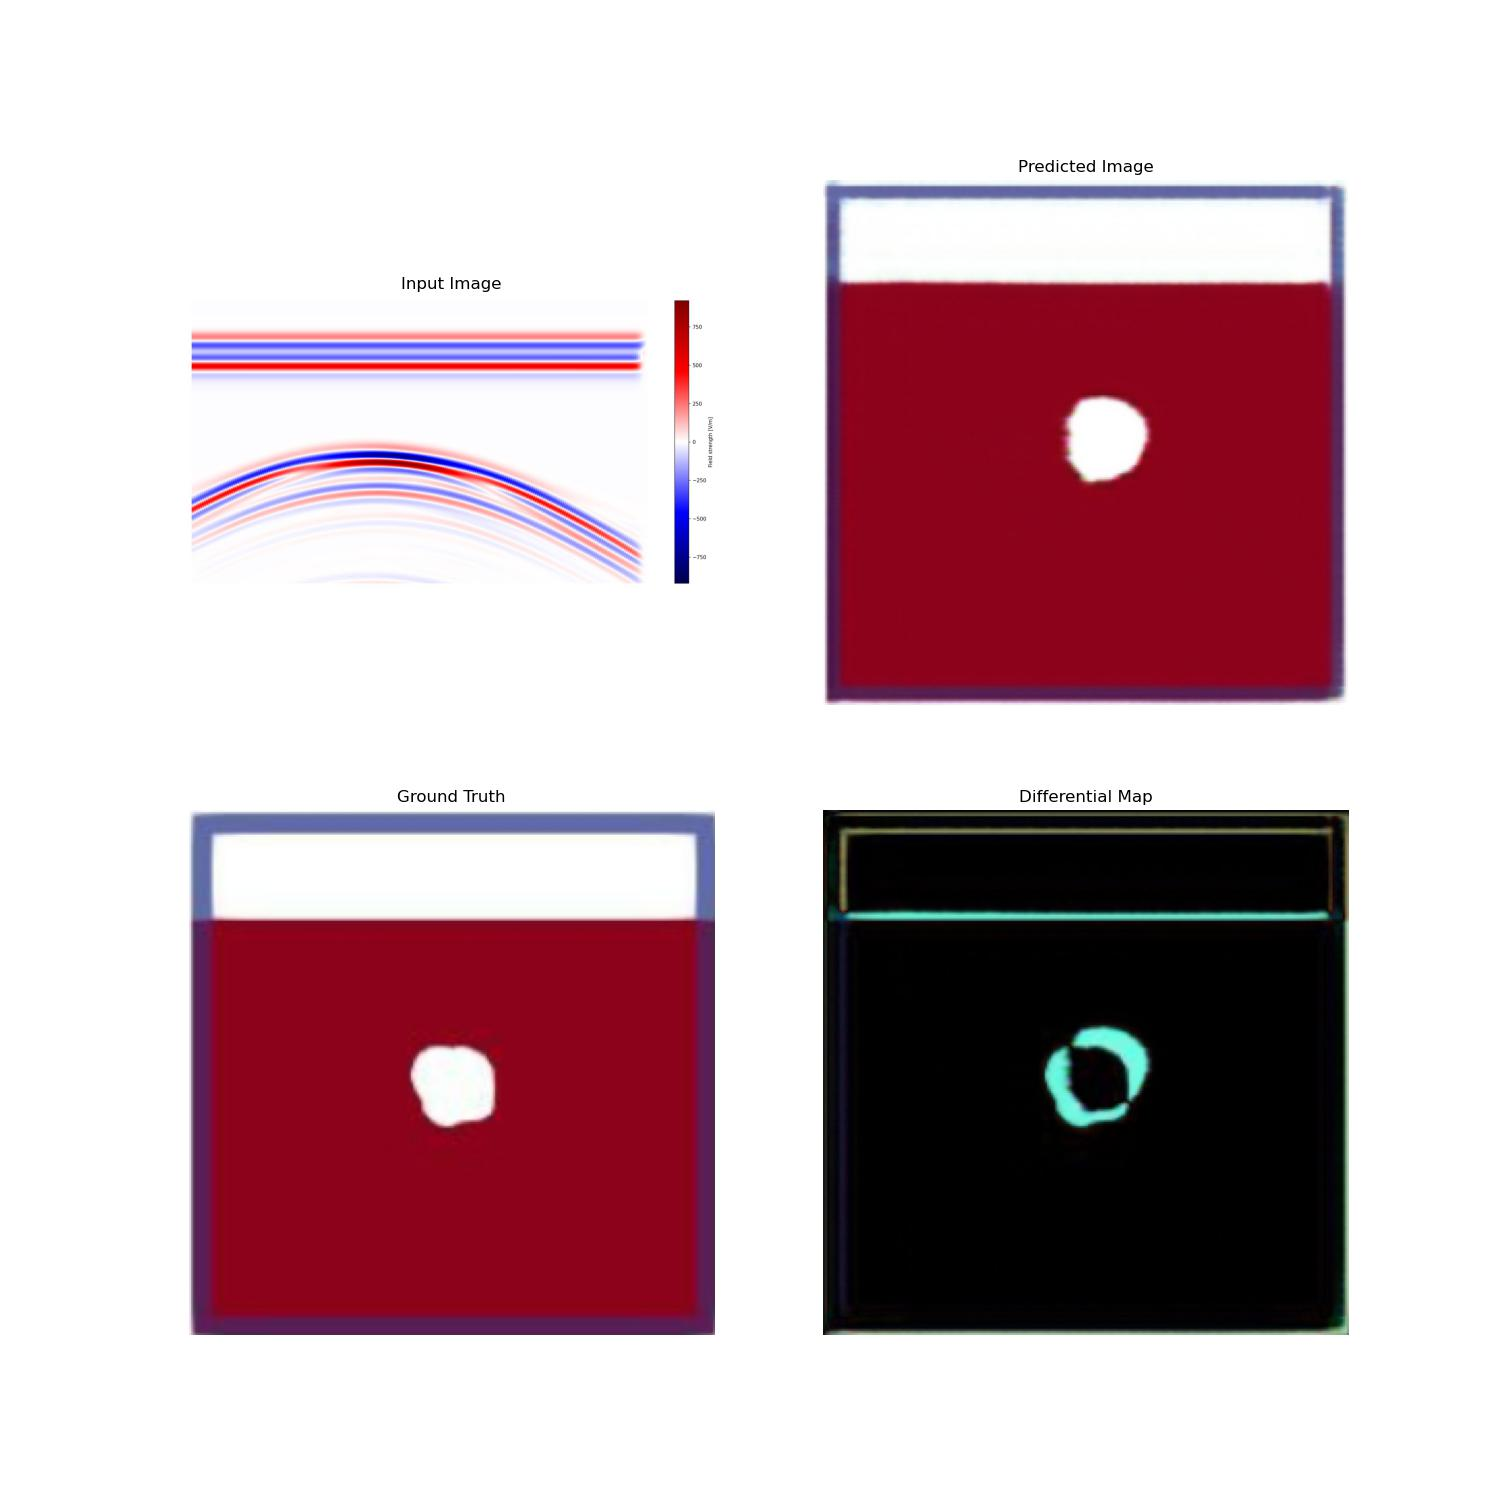
\includegraphics[scale=0.15]{gambar/diffMapSederhana.jpg}
  \caption{Evaluasi Visual Data Variasi Bentuk Sederhana}
  \label{fig:diffmapsederhana}
\end{figure}

Untuk variasi data dengan objek sederhana akan diambil data kedua karena memiliki nilai SSIM yang lebih buruk dari data lain. 
Evaluasi visual dari data dapat dilihat dari gambar \ref{fig:diffmapsederhana}.
Pada gambar evaluasi visual dapat dilihat bahwa irisan dari objek sintesis dengan objek asli cukup sedikit sehingga memiliki area error yang cukup luas. 
Hal ini menunjukkan bahwa posisi benda belum sepenuhnya dapat dideteksi oleh model.

\begin{figure}[ht]
  \centering
  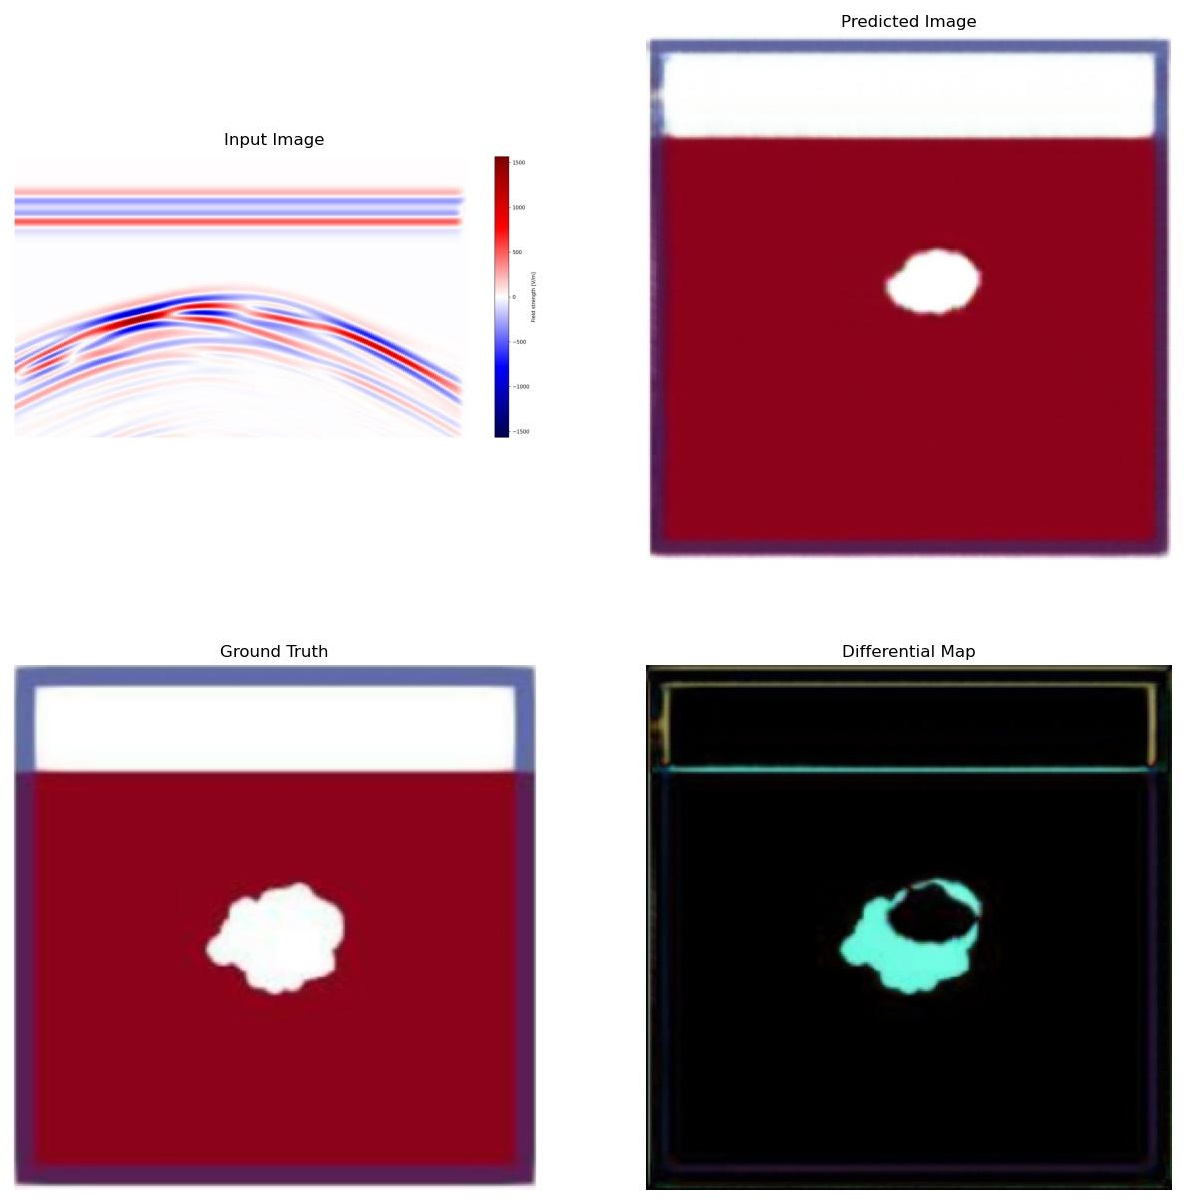
\includegraphics[scale=0.15]{gambar/diffMapKompleks.jpg}
  \caption{Evaluasi Visual Data Variasi Bentuk Kompleks}
  \label{fig:diffmapkompleks}
\end{figure}

Untuk variasi data dengan objek kompleks akan diambil data pertama karena memiliki nilai SSIM yang lebih baik dari data lain. 
Evaluasi visual dari data dapat dilihat dari gambar \ref{fig:diffmapkompleks}. 
Pada gambar evaluasi visual dapat dilihat bahwa irisan dari gambar sintesis dengan gambar asli merupakan gambar sintesis sepenuhnya. 
Hal ini menunjukkan bahwa model sudah bisa memprediksi posisi objek, namun masih belum bisa mensintesis ukuran objek dari objek berbentuk kompleks.

Pada variasi ukuran objek, terlihat untuk objek berukuran kecil memiliki rata-rata nilai evaluasi matriks yang lebih baik dari objek berukuran besar. 
Perbedaan rata-rata RMS dan MSE terlihat cukup jauh di antara kedua variasi data, sedangkan rata-rata SSIM terlihat cukup dekat. 
Namun, untuk beberapa data terdapat beberapa anomali, seperti data pertama dari variasi objek kecil dan data keempat dari objek besar. 

\begin{figure}[ht]
  \centering
  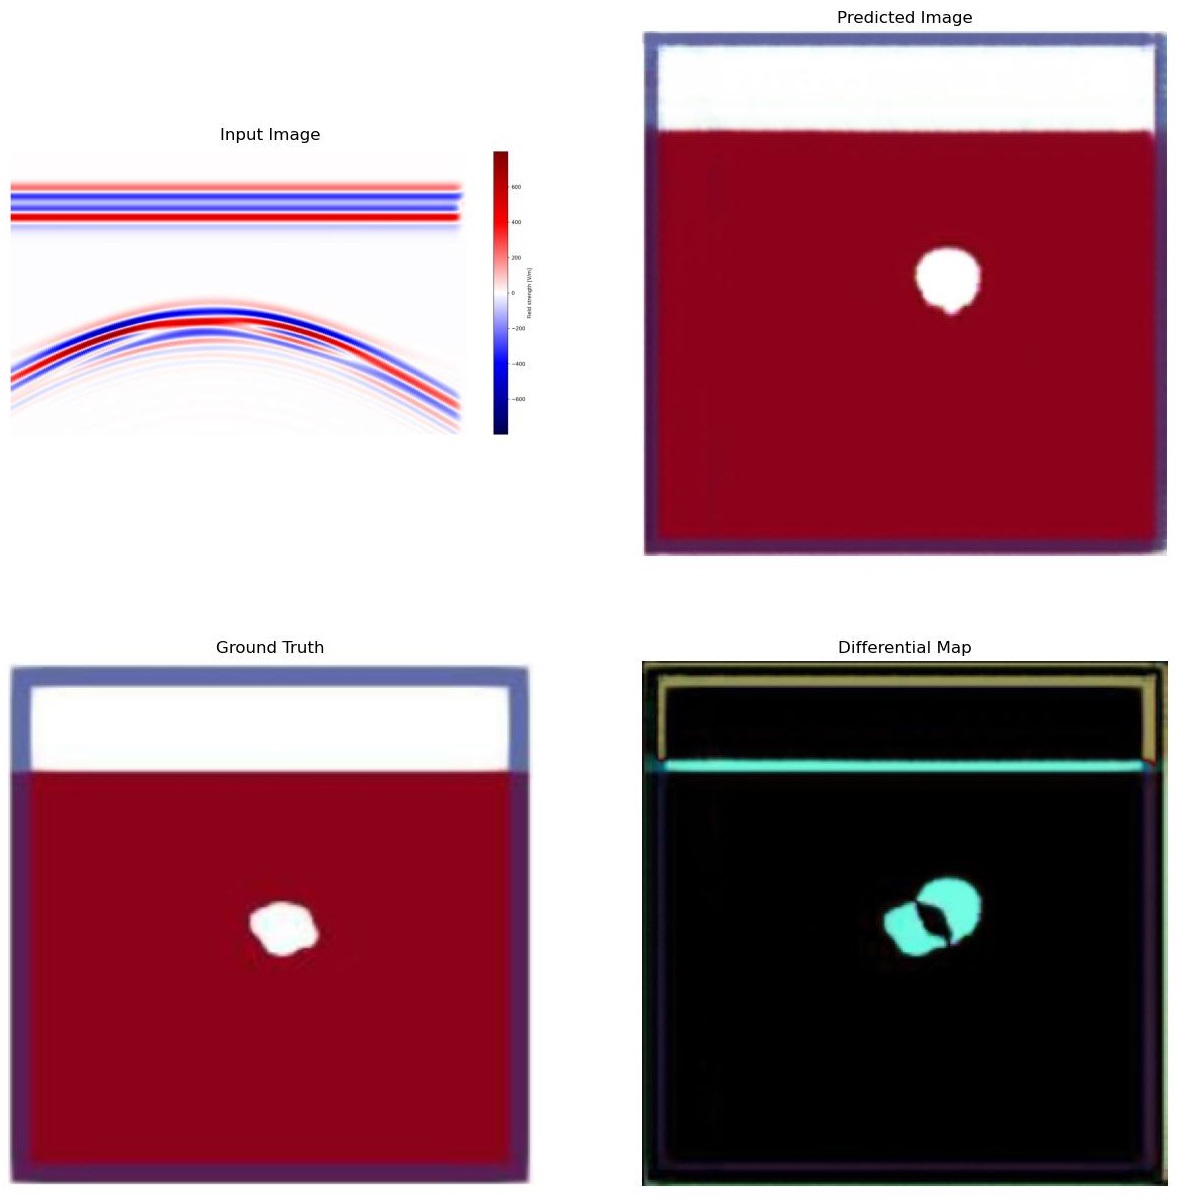
\includegraphics[scale=0.15]{gambar/diffMapKecil.jpg}
  \caption{Evaluasi Visual Data Variasi Ukuran Kecil}
  \label{fig:diffmapkecil}
\end{figure}

Data pertama dari variasi data dengan objek kecil memiliki nilai evaluasi matriks yang lebih buruk dari data lain. 
Evaluasi visual dari data dapat dilihat dari gambar \ref{fig:diffmapkecil}. 
Pada gambar evaluasi visual dapat dilihat bahwa irisan dari objek sintesis dengan objek asli cukup sedikit sehingga memiliki area error yang cukup luas. 
Hal ini menunjukkan bahwa posisi benda belum sepenuhnya dapat dideteksi oleh model.

\begin{figure}[ht]
  \centering
  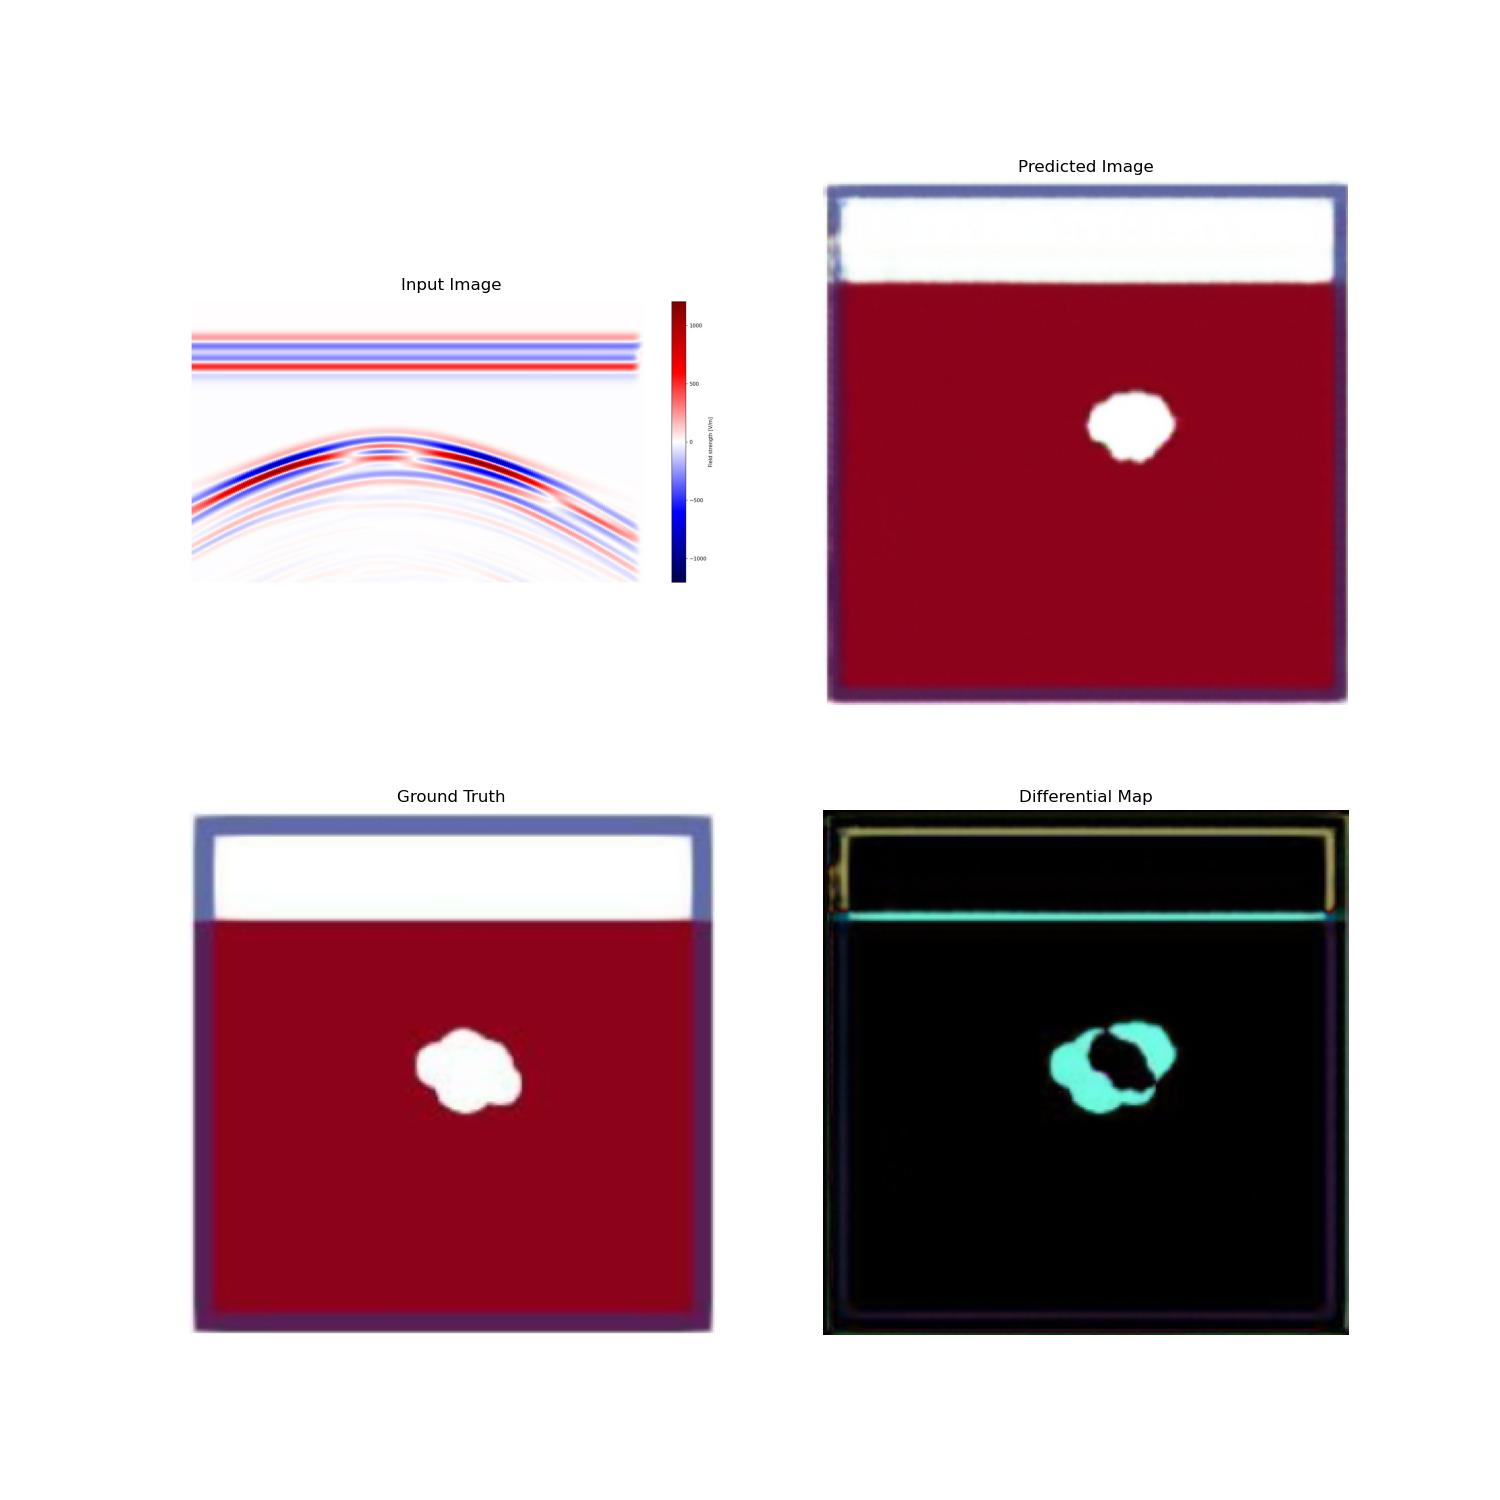
\includegraphics[scale=0.15]{gambar/diffMapBesar.jpg}
  \caption{Evaluasi Visual Data Variasi Ukuran Besar}
  \label{fig:diffmapbesar}
\end{figure}

Data keempat dari variasi data dengan objek besar karena memiliki nilai evaluasi matriks yang lebih baik dari data lain. 
Evaluasi visual dari data dapat dilihat dari gambar \ref{fig:diffmapbesar}. 
Pada gambar evaluasi visual dapat dilihat bahwa irisan dari objek sintesis dengan objek asli cukup luas sehingga memiliki area error yang cukup sedikit. 
Hal ini menunjukkan bahwa posisi beserta ukuran benda hampir dapat dideteksi oleh model. \\

Pada variasi posisi objek, terlihat untuk objek dengan posisi dekat dengan permukaan memiliki rata-rata nilai evaluasi matriks yang lebih baik dari objek dengan posisi jauh dengan permukaan. 
Perbedaan rata-rata evaluasi matriks terlihat cukup dekat di antara kedua variasi data, sedangkan rata-rata SSIM terlihat cukup jauh. 
Namun, untuk beberapa data terdapat beberapa anomali, seperti data ketiga dari variasi posisi objek dekat dari permukaan dan data ketiga dari variasi posisi objek jauh dari permukaan. 

\begin{figure}[ht]
  \centering
  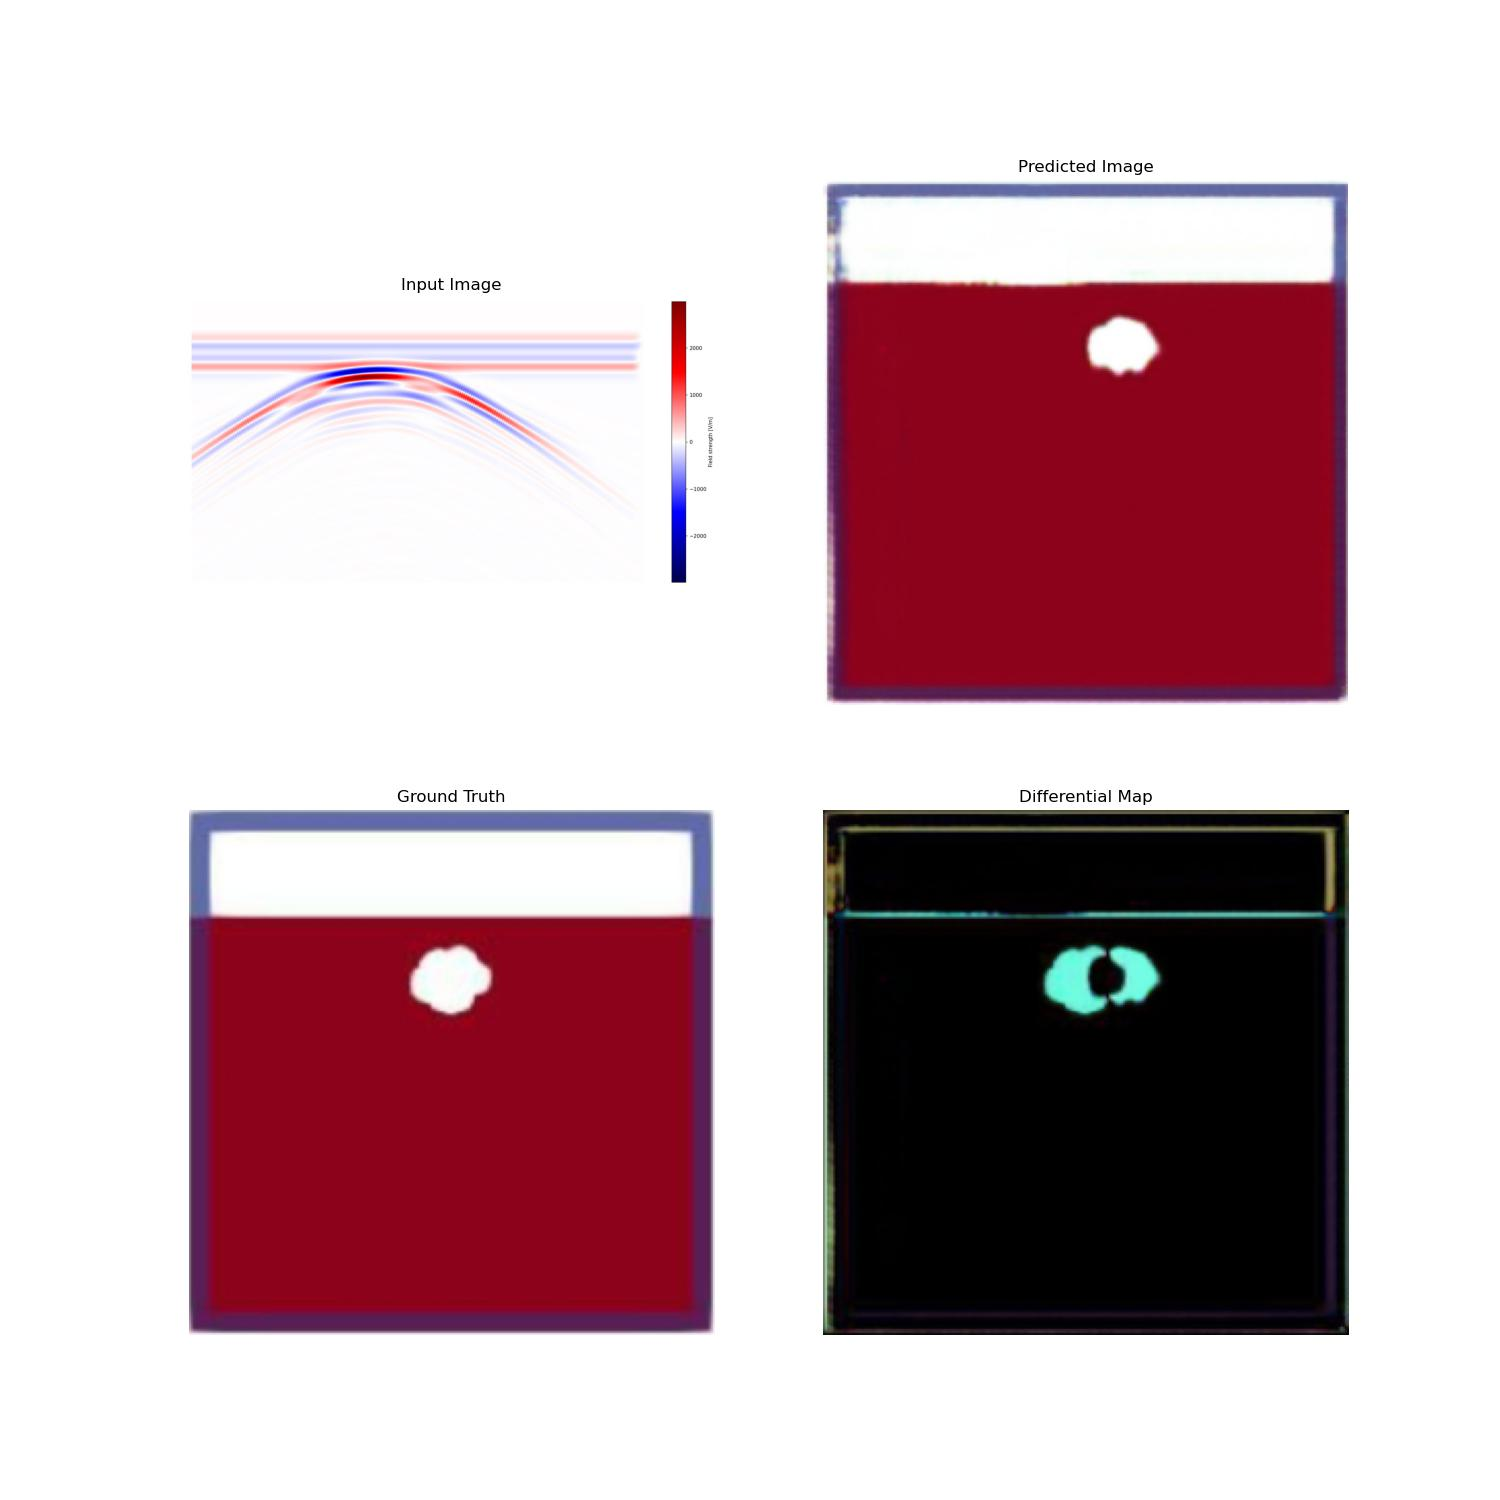
\includegraphics[scale=0.15]{gambar/diffMapDangkal.jpg}
  \caption{Evaluasi Visual Data Variasi Posisi Dekat dengan Permukaan}
  \label{fig:diffmapdangkal}
\end{figure}

Data ketiga dari variasi posisi objek dekat dengan permukaan memiliki nilai evaluasi matriks yang lebih buruk dari data lain. 
Evaluasi visual dari data dapat dilihat dari gambar \ref{fig:diffmapdangkal}. 
Pada gambar evaluasi visual dapat dilihat bahwa irisan dari objek sintesis dengan objek asli cukup sedikit sehingga memiliki area error yang cukup luas . 
Hal ini menunjukkan bahwa posisi beserta ukuran benda belum sepenuhnya dapat dideteksi oleh model.

\begin{figure}[ht]
  \centering
  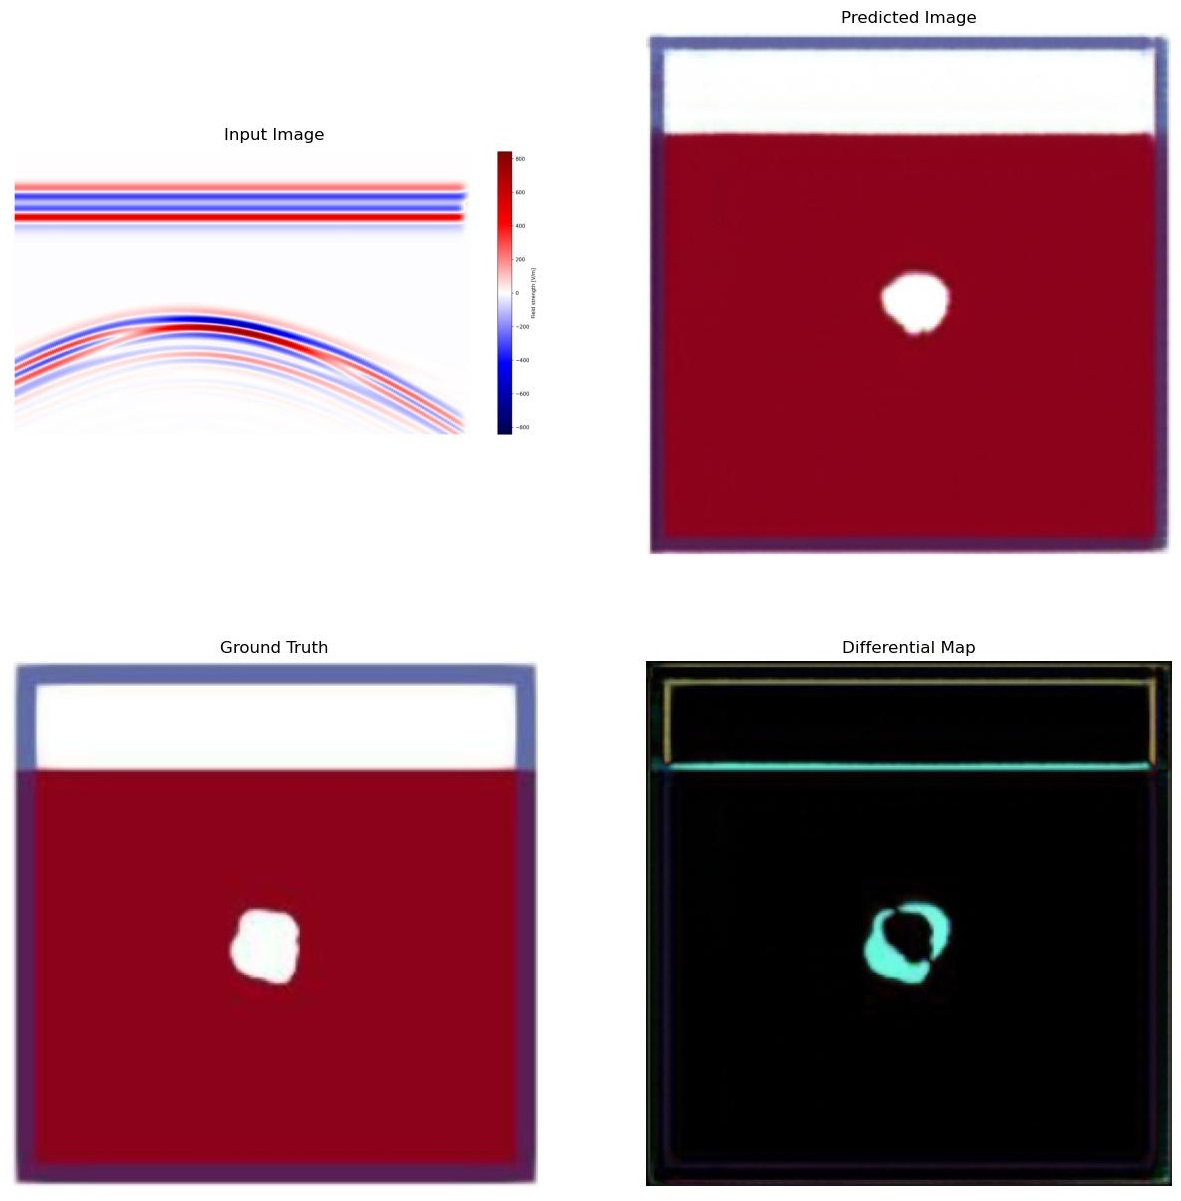
\includegraphics[scale=0.15]{gambar/diffMapDalam.jpg}
  \caption{Evaluasi Visual Data Variasi Posisi Jauh dengan Permukaan}
  \label{fig:diffmapdalam}
\end{figure}

Data ketiga dari variasi posisi objek jauh dengan permukaan memiliki nilai evaluasi matriks yang lebih buruk dari data lain. 
Evaluasi visual dari data dapat dilihat dari gambar \ref{fig:diffmapdalam}. 
Pada gambar evaluasi visual dapat dilihat bahwa irisan dari objek sintesis dengan objek asli cukup sedikit sehingga memiliki area error yang cukup luas. 
Hal ini menunjukkan bahwa posisi beserta ukuran benda belum sepenuhnya dapat dideteksi oleh model.  

Secara keseluruhan evaluasi matriks test data, diperoleh rata-rata RMS = 27.177, MSE = 1351.405, dan SSIM = 0.833. 
Tidak ada standar nilai RMS, MSE, dan SSIM yang bersifat universal atau mutlak untuk menentukan apakah suatu gambar dianggap baik atau buruk. 
Oleh karena itu, nilai rata-rata ini digunakan sebagai standar kemampuan model dalam menghasilkan data setiap variasinya.

Untuk variasi yang nilai rata-rata RMS dan MSE-nya lebih kecil dari nilai rata-rata RMS dan MSE total, dapat dikatakan intensitas piksel antara gambar yang disintesis dengan gambar asli hampir sama. 
Variasi tersebut diantaranya variasi bentuk regular lingkaran, bentuk regular segi empat, ukuran objek kecil, posisi objek dekat dari permukaan, dan posisi objek jauh dari permukaan. 
Sebaliknya, untuk variasi yang nilai rata-rata RMS dan MSE-nya lebih besar dari nilai rata-rata RMS dan MSE total, dapat dikatakan intensitas piksel antara gambar yang disintesis dengan gambar asli cukup jauh. 
Variasi tersebut diantaranya variasi bentuk objek sederhana, bentuk objek kompleks, dan ukuran objek besar.

Untuk variasi yang nilai rata-rata SSIM-nya lebih besar dari nilai rata-rata SSIM total, dapat dikatakan kesamaan struktural antara gambar yang disintesis dengan gambar asli hampir sama. 
Variasi tersebut diantaranya variasi bentuk regular lingkaran, bentuk regular segi empat, dan posisi objek jauh dari permukaan. 
Sebaliknya, untuk variasi yang nilai rata-rata SSIM-nya lebih kecil dari nilai rata-rata SSIM total, dapat dikatakan kesamaan struktural antara gambar yang disintesis dengan gambar asli cukup jauh. 
Variasi tersebut diantaranya variasi bentuk objek sederhana, bentuk objek kompleks, ukuran objek kecil, ukuran objek besar, dan posisi objek jauh dari permukaan.

\cleardoublepage

% Bab 5 penutup
\chapter{PENUTUP}
\label{chap:penutup}

% Ubah bagian-bagian berikut dengan isi dari penutup

\section{Kesimpulan}
\label{sec:kesimpulan}

Berdasarkan hasil pengujian yang \lipsum[1][1-3] sebagai berikut:

\begin{enumerate}[nolistsep]

  \item Pembuatan \lipsum[2][1-3]

  \item \lipsum[2][4-6]

  \item \lipsum[2][7-10]

\end{enumerate}

\section{Saran}
\label{chap:saran}

Untuk pengembangan lebih lanjut pada \lipsum[1][1-3] antara lain:

\begin{enumerate}[nolistsep]

  \item Memperbaiki \lipsum[2][1-3]

  \item \lipsum[2][4-6]

  \item \lipsum[2][7-10]

\end{enumerate}

\cleardoublepage

\chapter*{DAFTAR PUSTAKA}
\addcontentsline{toc}{chapter}{DAFTAR PUSTAKA}
\renewcommand\refname{}
\vspace{2ex}
\renewcommand{\bibname}{}
\begingroup
\def\chapter*#1{}
\printbibliography
\endgroup
\cleardoublepage

% Biografi penulis
\begin{center}
  \Large
  \textbf{BIOGRAFI PENULIS}
\end{center}

\addcontentsline{toc}{chapter}{BIOGRAFI PENULIS}

\vspace{2ex}

\begin{wrapfigure}{L}{0.3\textwidth}
  \centering
  \vspace{-3ex}
  % Ubah file gambar berikut dengan file foto dari mahasiswa
  
\includegraphics[width=0.3\textwidth]{gambar/elon.jpg}
  \vspace{-4ex}
\end{wrapfigure}

% Ubah kalimat berikut dengan biografi dari mahasiswa
\name{}, lahir pada \lipsum[1]

\lipsum[2]

\cleardoublepage

\end{document}
